% Template for PLoS
% Version 3.5 March 2018
%
% % % % % % % % % % % % % % % % % % % % % %
%
% -- IMPORTANT NOTE
%
% This template contains comments intended 
% to minimize problems and delays during our production 
% process. Please follow the template instructions
% whenever possible.
%
% % % % % % % % % % % % % % % % % % % % % % % 
%
% Once your paper is accepted for publication, 
% PLEASE REMOVE ALL TRACKED CHANGES in this file 
% and leave only the final text of your manuscript. 
% PLOS recommends the use of latexdiff to track changes during review, as this will help to maintain a clean tex file.
% Visit https://www.ctan.org/pkg/latexdiff?lang=en for info or contact us at latex@plos.org.
%
%
% There are no restrictions on package use within the LaTeX files except that 
% no packages listed in the template may be deleted.
%
% Please do not include colors or graphics in the text.
%
% The manuscript LaTeX source should be contained within a single file (do not use \input, \externaldocument, or similar commands).
%
% % % % % % % % % % % % % % % % % % % % % % %
%
% -- FIGURES AND TABLES
%
% Please include tables/figure captions directly after the paragraph where they are first cited in the text.
%
% DO NOT INCLUDE GRAPHICS IN YOUR MANUSCRIPT
% - Figures should be uploaded separately from your manuscript file. 
% - Figures generated using LaTeX should be extracted and removed from the PDF before submission. 
% - Figures containing multiple panels/subfigures must be combined into one image file before submission.
% For figure citations, please use "Fig" instead of "Figure".
% See http://journals.plos.org/plosone/s/figures for PLOS figure guidelines.
%
% Tables should be cell-based and may not contain:
% - spacing/line breaks within cells to alter layout or alignment
% - do not nest tabular environments (no tabular environments within tabular environments)
% - no graphics or colored text (cell background color/shading OK)
% See http://journals.plos.org/plosone/s/tables for table guidelines.
%
% For tables that exceed the width of the text column, use the adjustwidth environment as illustrated in the example table in text below.
%
% % % % % % % % % % % % % % % % % % % % % % % %
%
% -- EQUATIONS, MATH SYMBOLS, SUBSCRIPTS, AND SUPERSCRIPTS
%
% IMPORTANT
% Below are a few tips to help format your equations and other special characters according to our specifications. For more tips to help reduce the possibility of formatting errors during conversion, please see our LaTeX guidelines at http://journals.plos.org/plosone/s/latex
%
% For inline equations, please be sure to include all portions of an equation in the math environment.  For example, x$^2$ is incorrect; this should be formatted as $x^2$ (or $\mathrm{x}^2$ if the romanized font is desired).
%
% Do not include text that is not math in the math environment. For example, CO2 should be written as CO\textsubscript{2} instead of CO$_2$.
%
% Please add line breaks to long display equations when possible in order to fit size of the column. 
%
% For inline equations, please do not include punctuation (commas, etc) within the math environment unless this is part of the equation.
%
% When adding superscript or subscripts outside of brackets/braces, please group using {}.  For example, change "[U(D,E,\gamma)]^2" to "{[U(D,E,\gamma)]}^2". 
%
% Do not use \cal for caligraphic font.  Instead, use \mathcal{}
%
% % % % % % % % % % % % % % % % % % % % % % % % 
%
% Please contact latex@plos.org with any questions.
%
% % % % % % % % % % % % % % % % % % % % % % % %

\documentclass[10pt,letterpaper]{article}
\usepackage[top=0.85in,left=2.75in,footskip=0.75in]{geometry}

% amsmath and amssymb packages, useful for mathematical formulas and symbols
\usepackage{amsmath,amssymb}

% Use adjustwidth environment to exceed column width (see example table in text)
\usepackage{changepage}

% Use Unicode characters when possible
\usepackage[utf8x]{inputenc}

% textcomp package and marvosym package for additional characters
\usepackage{textcomp,marvosym}

% cite package, to clean up citations in the main text. Do not remove.
\usepackage{cite}

% Use nameref to cite supporting information files (see Supporting Information section for more info)
\usepackage{nameref,hyperref}

% line numbers
\usepackage[right]{lineno}

% ligatures disabled
\usepackage{microtype}
\DisableLigatures[f]{encoding = *, family = * }

% color can be used to apply background shading to table cells only
\usepackage[table]{xcolor}

% array package and thick rules for tables
\usepackage{array}

% create "+" rule type for thick vertical lines
\newcolumntype{+}{!{\vrule width 2pt}}

% create \thickcline for thick horizontal lines of variable length
\newlength\savedwidth
\newcommand\thickcline[1]{%
  \noalign{\global\savedwidth\arrayrulewidth\global\arrayrulewidth 2pt}%
  \cline{#1}%
  \noalign{\vskip\arrayrulewidth}%
  \noalign{\global\arrayrulewidth\savedwidth}%
}

% \thickhline command for thick horizontal lines that span the table
\newcommand\thickhline{\noalign{\global\savedwidth\arrayrulewidth\global\arrayrulewidth 2pt}%
\hline
\noalign{\global\arrayrulewidth\savedwidth}}


% Remove comment for double spacing
%\usepackage{setspace} 
%\doublespacing

% Text layout
\raggedright
\setlength{\parindent}{0.5cm}
\textwidth 5.25in 
\textheight 8.75in

% Bold the 'Figure #' in the caption and separate it from the title/caption with a period
% Captions will be left justified
\usepackage[aboveskip=1pt,labelfont=bf,labelsep=period,justification=raggedright,singlelinecheck=off]{caption}
\renewcommand{\figurename}{Fig}

% Use the PLoS provided BiBTeX style
\bibliographystyle{plos2015}

% Remove brackets from numbering in List of References
\makeatletter
\renewcommand{\@biblabel}[1]{\quad#1.}
\makeatother



% Header and Footer with logo
\usepackage{lastpage,fancyhdr,graphicx}
\usepackage{epstopdf}
%\pagestyle{myheadings}
\pagestyle{fancy}
\fancyhf{}
%\setlength{\headheight}{27.023pt}
%\lhead{
\includegraphics[width=2.0in]{PLOS-submission.eps}}
\rfoot{\thepage/\pageref{LastPage}}
\renewcommand{\headrulewidth}{0pt}
\renewcommand{\footrule}{\hrule height 2pt \vspace{2mm}}
\fancyheadoffset[L]{2.25in}
\fancyfootoffset[L]{2.25in}
\lfoot{\today}

%% Include all macros below

\newcommand{\sticky}{proglobular~}
\usepackage{makecell}
\usepackage{multirow}

\renewcommand\theadalign{bc}
\renewcommand\theadfont{\bfseries}
\renewcommand\theadgape{\Gape[4pt]}
\renewcommand\cellgape{\Gape[4pt]}

%% END MACROS SECTION



\begin{document}
\vspace*{0.2in}

% Title must be 250 characters or less.
\begin{flushleft}
{\Large
\textbf\newline{Disease causing mutations are found in hydrophobic regions in both ordered and disordered proteins} % Please use "sentence case" for title and headings (capitalize only the first word in a title (or heading), the first word in a subtitle (or subheading), and any proper nouns).
}
\newline
% Insert author names, affiliations and corresponding author email (do not include titles, positions, or degrees).
\\
Ruchi Lohia\textsuperscript{1},
Matt Hansen\textsuperscript{2},
Grace Brannigan\textsuperscript{1,3*},
\\
\bigskip
\textbf{1} Center for Computational and Integrative Biology, Rutgers University, Camden, NJ, USA
\\
\textbf{2}  Department of Genetics and Center of Excellence in Environmental Toxicology, University of Pennsylvania 
\\
\textbf{3} Department of Physics, Rutgers University, Camden, NJ, USA
\\
\bigskip

% Insert additional author notes using the symbols described below. Insert symbol callouts after author names as necessary.
% 
% Remove or comment out the author notes below if they aren't used.
%
% Primary Equal Contribution Note
%\Yinyang These authors contributed equally to this work.

% Additional Equal Contribution Note
% Also use this double-dagger symbol for special authorship notes, such as senior authorship.
%\ddag These authors also contributed equally to this work.

% Current address notes
%\textcurrency Current Address: Dept/Program/Center, Institution Name, City, State, Country % change symbol to "\textcurrency a" if more than one current address note
% \textcurrency b Insert second current address 
% \textcurrency c Insert third current address

% Deceased author note
%\dag Deceased

% Group/Consortium Author Note
%\textpilcrow Membership list can be found in the Acknowledgments section.

% Use the asterisk to denote corresponding authorship and provide email address in note below.
* grace.brannigan@rutgers.edu(GB)

\end{flushleft}


% Please keep the abstract below 300 words
\section*{Abstract}


% Please keep the Author Summary between 150 and 200 words
% Use first person. PLOS ONE authors please skip this step. 
% Author Summary not valid for PLOS ONE submissions.   
\section*{Author summary} 

%%%%%%%%%%%%%%%%%%%%%%%%%%%%%%%%%%%%%%%%%%%%%%%%%%%%%%%%%%%%%%%%%%%%%
%% Start the main part of the manuscript here.
%%%%%%%%%%%%%%%%%%%%%%%%%%%%%%%%%%%%%%%%%%%%%%%%%%%%%%%%%%%%%%%%%%%%%

\section*{Introduction}

The physiological significance of intrinsically disordered proteins (IDPs), which can explore a wide range of conformational ensembles in their functional form, is now well-established~\cite {Uversky2013a,Panchenko2015,Ward2004a,Dyson2005a}. More than 33\% of eukaryotic proteins contain disordered regions longer than 30 residues\cite{Ward2004a}, many of which are involved in critical biological functions, including transcriptional regulation and cell signaling\cite{Dunker2005}. Long intrinsically disordered regions are particularly abundant among cancer and neurodegenerative-associated proteins\cite{Habchi2014,Babu2011}.  

IDP amino-acid sequences tend to be low complexity and include numerous charged residues, often in long repeats~\cite{Uversky2013a}. In contrast to ordered proteins, in which a complex sequence encodes a well-defined tertiary structure, an IDP sequence determines a heterogeneous conformational ensemble. 

Although IDP sequences are low-complexity and do not encode a well-defined structure, single residue substitutions can still have functional effects that are significant for the organism. More than 20\% of disease-associated missense single nucelotide polymorphisms (SNPs) are found in IDPs\cite{Vacic2012a}; although detectable, the relatively subtle functional effects may lead to relatively weak selection pressure, whether positive or negative, allowing the mutation to persist at high frequencies within a population. Numerous structural and simulation studies~\cite{Larini2013b,Ganguly2015,Viet2014a,Viet2013,Truong2014a,Zhan2013a,Xu2013a} have demonstrated clear effects of single charged-residue insertion, deletion, or substitutions on conformational ensemble and aggregation of IDPs monomers. Single charged residue mutations or post translational modifications that change charges will affect the sequence electrostatics predicted to determine ensemble properties simply from statistical physics models, and in short-chains, can also induce qualitative changes by changing the appropriate regime~\cite{Das2015,Larini2013b,Bah2016,He2015}. Locally, such mutations can modulate residual secondary structure preferences via forming or breaking local salt-bridges or by introducing helix breaking residues~\cite{AlexanderConicella2016,Ganguly2015,Zhan2013a}. 

For IDPs with a relatively low fraction of charged residues, typical of the Janus region of the state diagram proposed by Das and Pappu\cite{Das2015,Das2013a}, more subtle differences among neutral amino-acids play an increasingly important role in determining the ensemble. More than 15\% of disease-associated IDP polymorphisms are substitutions between two charge-neutral residues~\cite{Vacic2012a}. The extent to which such substitutions in IDPs can affect non-local aspects of the conformational ensemble is uncertain; these substitutions directly affect short-range interactions, and structure-based coupling between distant residues in IDPs is expected to be weak. Nonetheless, correlations between secondary structure of distant residues has been frequently observed in IDPs~\cite{Ganguly2015,Iesmantavicius2013}; for example, several cancer mutations in transactivation domain of tumor suppressor p53 can lead to helicity changes in residues sequentially far away from the mutation sites~\cite{Ganguly2015}.

\section{Results and discussion}

\subsection*{SNP distributions in ordered and disordered regions}
Among the total 58,645 SNPs analyzed, 47.6\% lies in disordered regions and remaining 52.3\% in ordered regions. When the SNPs were further broken down into Disease-associated (DA) and not-disease-associated (NDA), we find that 64.2\% of DA are found in ordered region and 35.8\% are found in disordered region (Fig~\ref{fig1}). As observed previously~\cite{Vacic2012a}, we find that disease associated mutations are enriched by 0.49 fold in ordered regions and 0.37 fold depleted depleted in disordered regions relative to the not-disease associated SNPs (Fig~\ref{fig1}). 

\begin{figure}[!ht]
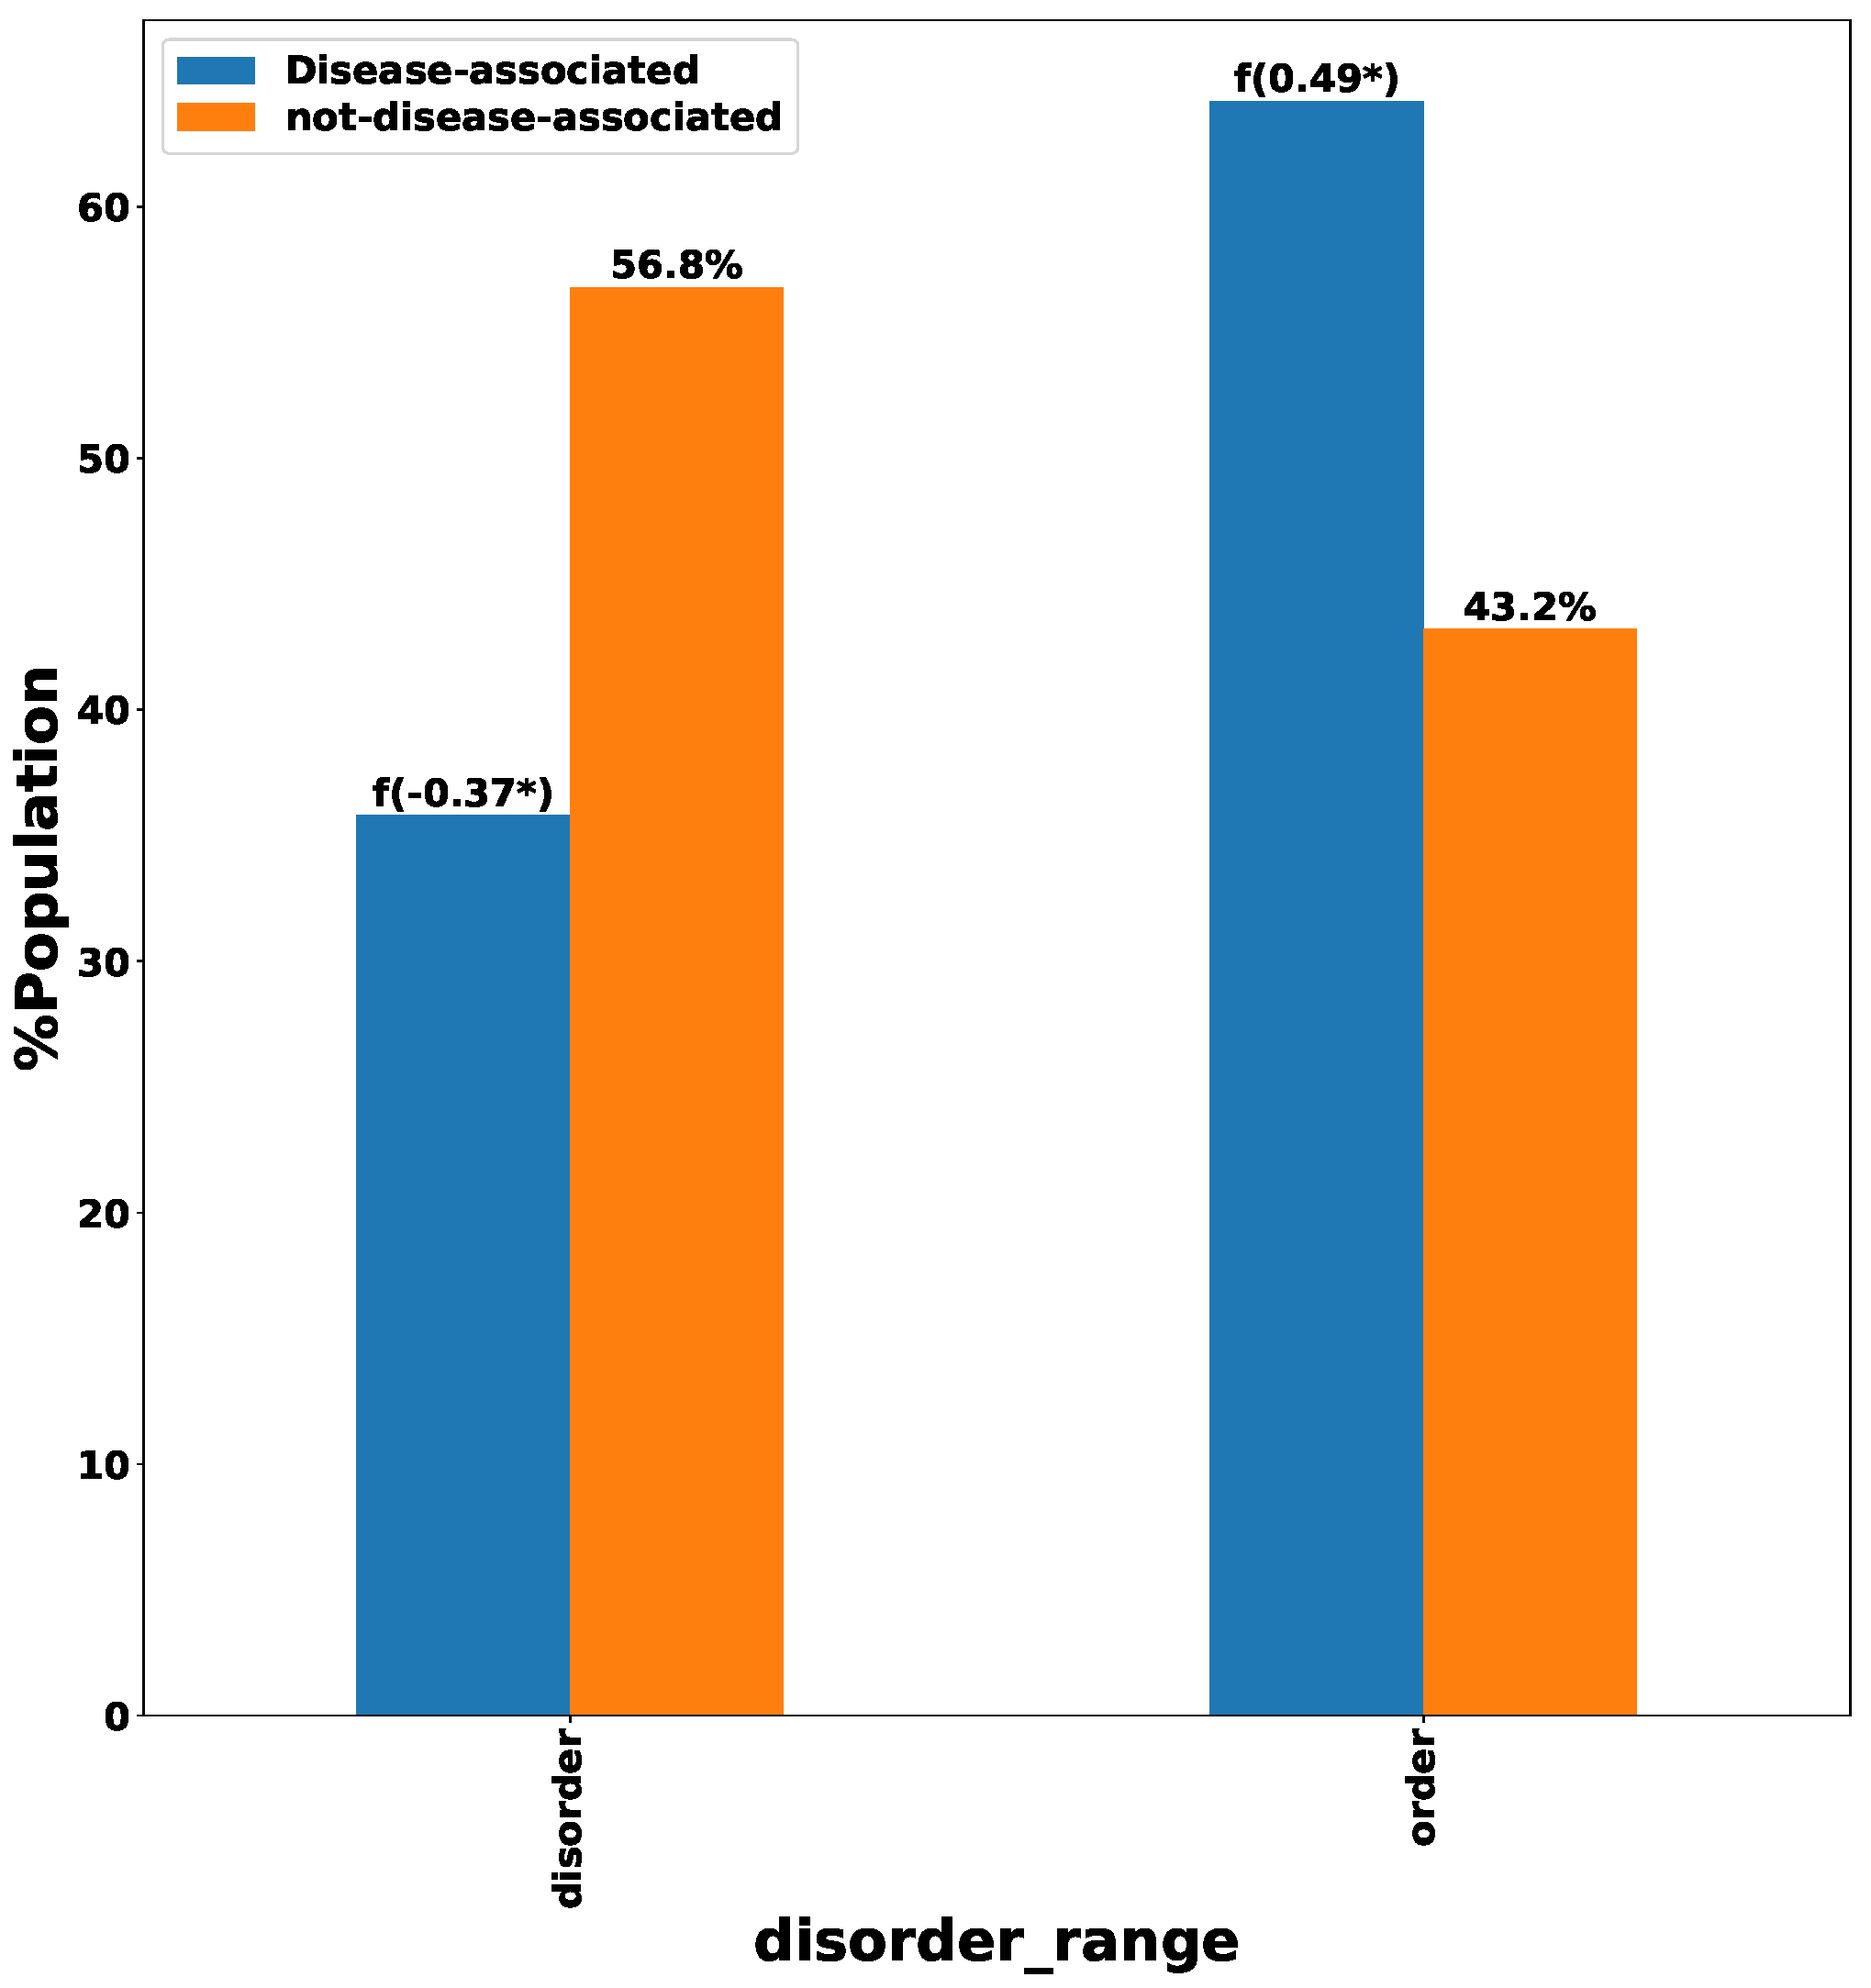
\includegraphics[scale=0.1,width=0.5\textwidth,trim={0 0cm 0 0cm},clip]{./figures/order_vs_disorder_SNP.pdf}
\caption{{\bf Disease mutations have higher frequency in ordered regions.} The population of DA SNPs (blue bar) and NDA SNPs (orange bar) in ordered region and disordered region. The expected population for DA SNPs in ordered and disordered set from NDA SNPs is labeled at the top of orange bars. Fold enrichment in DA SNPs when compared with not-disease-associated SNPs is annotated in the plot as well with f. If p-value from the binomial test is $<$ .005, the enrichment is marked with star. }
\label{fig1} 
\end{figure}


\subsection*{Type of SNP distribution}
 About 50\% of the disease causing SNPs in both ordered and disordered proteins are charge-neutral (Fig~\ref{fig2}).  

\begin{figure}[!ht]
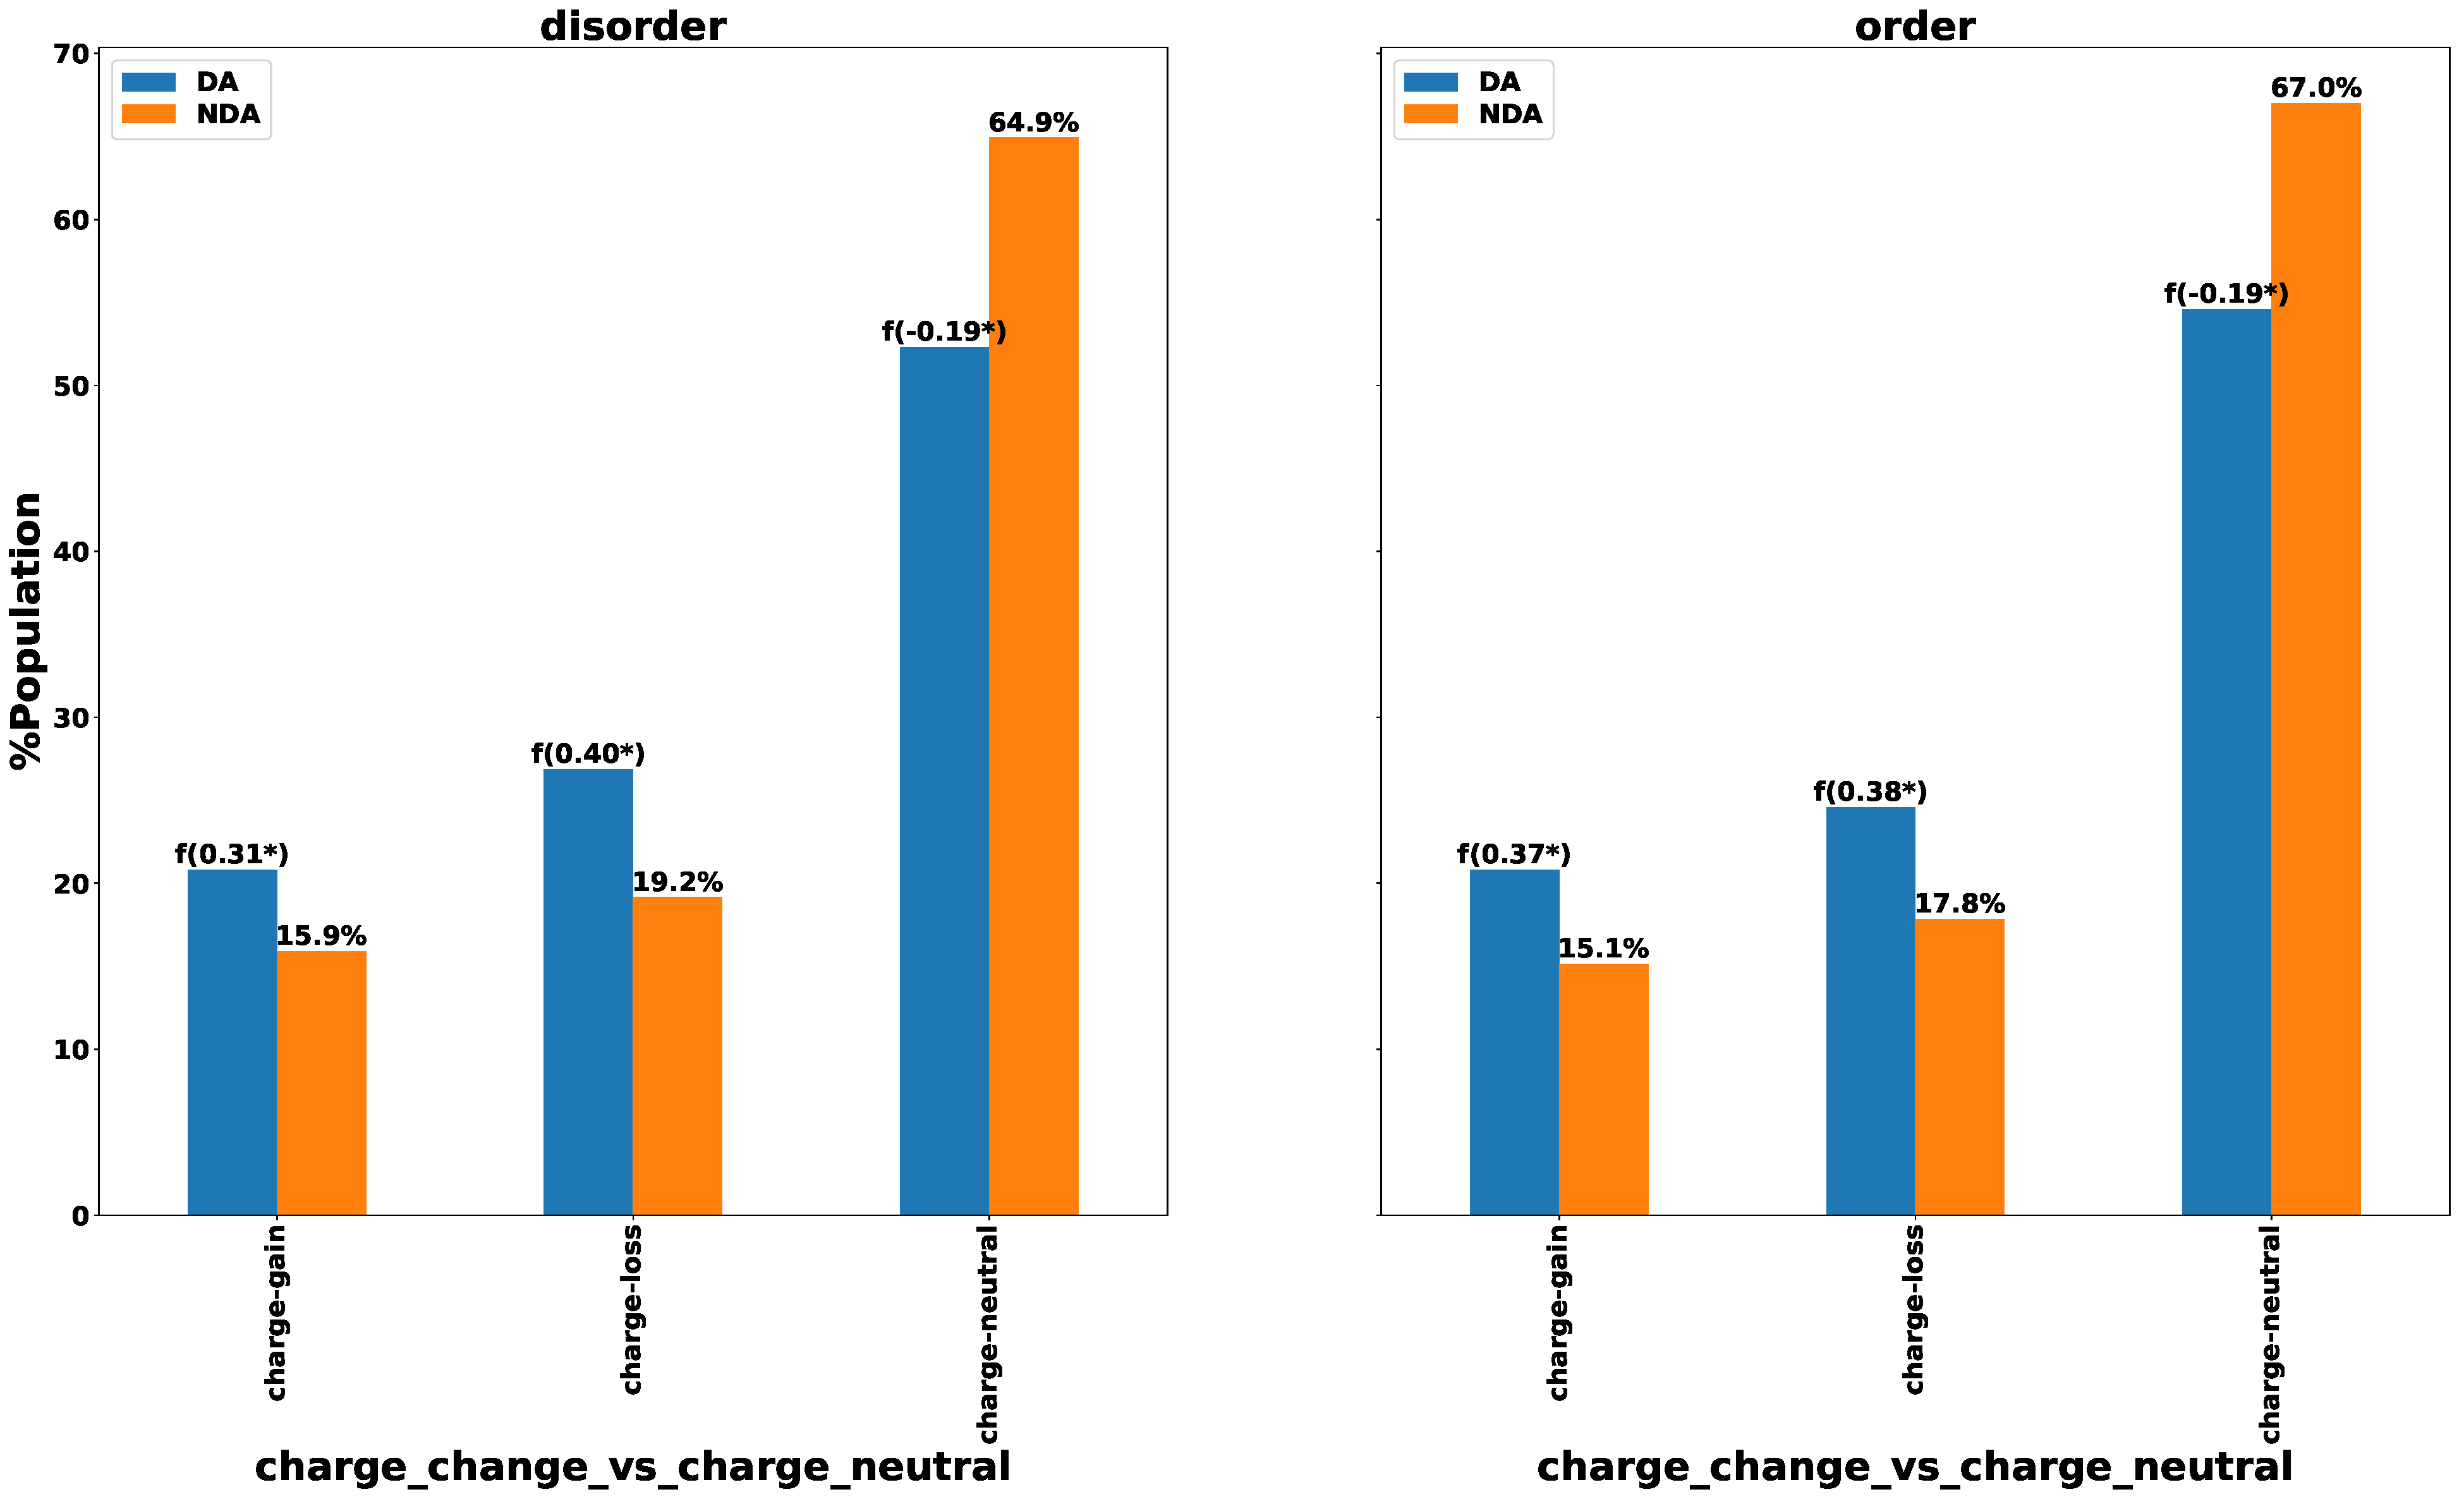
\includegraphics[scale=0.1,width=0.8\textwidth,trim={0 0cm 0 0cm},clip]{./figures/charge_vs_no_charge_order_vs_disorder_SNP.pdf}
\caption{{\bf DA SNPs are more enriched in gain/loss of charge.} We divided each SNP into three categories: charge-neutral SNPs, SNPs that lead to charge gain and SNPs that lead to charge loss. We then plotted the population for DA and NDA SNPS in ordered and disordered proteins in each category. We find that 50\% of the disease causing SNPs in both ordered and disordered proteins are charge-neutral. Fold enrichment in DA SNPs when compared with NDA SNPs is annotated in the plot as well with f. If p-value from the binomial test is $<$ .005, the enrichment is marked with star. DA SNPs are enriched in charge-gain or charge-loss but depleted in charge-neutral SNPs relative to the NDA SNPs. }
\label{fig2} 
\end{figure}

\subsection*{DA SNPs are enriched in hydrophobic regions}
We looked at the hydrophobicity distribution of SNP residue and it's neighboring residue (window size 3,5 and 15). $<$H$>$ at window size 3 is defined as the Hydropathy score of \begin{equation}\frac{H_{i}+H_{i-1}+H_{i+1} }{3}\label{eq:bond}\end{equation}
 where i is the SNP residue. We find that the DA SNP is more enriched in hydrophobic regions in both ordered and disordered proteins relative to the NDA SNPs . 

\begin{figure}[!ht]
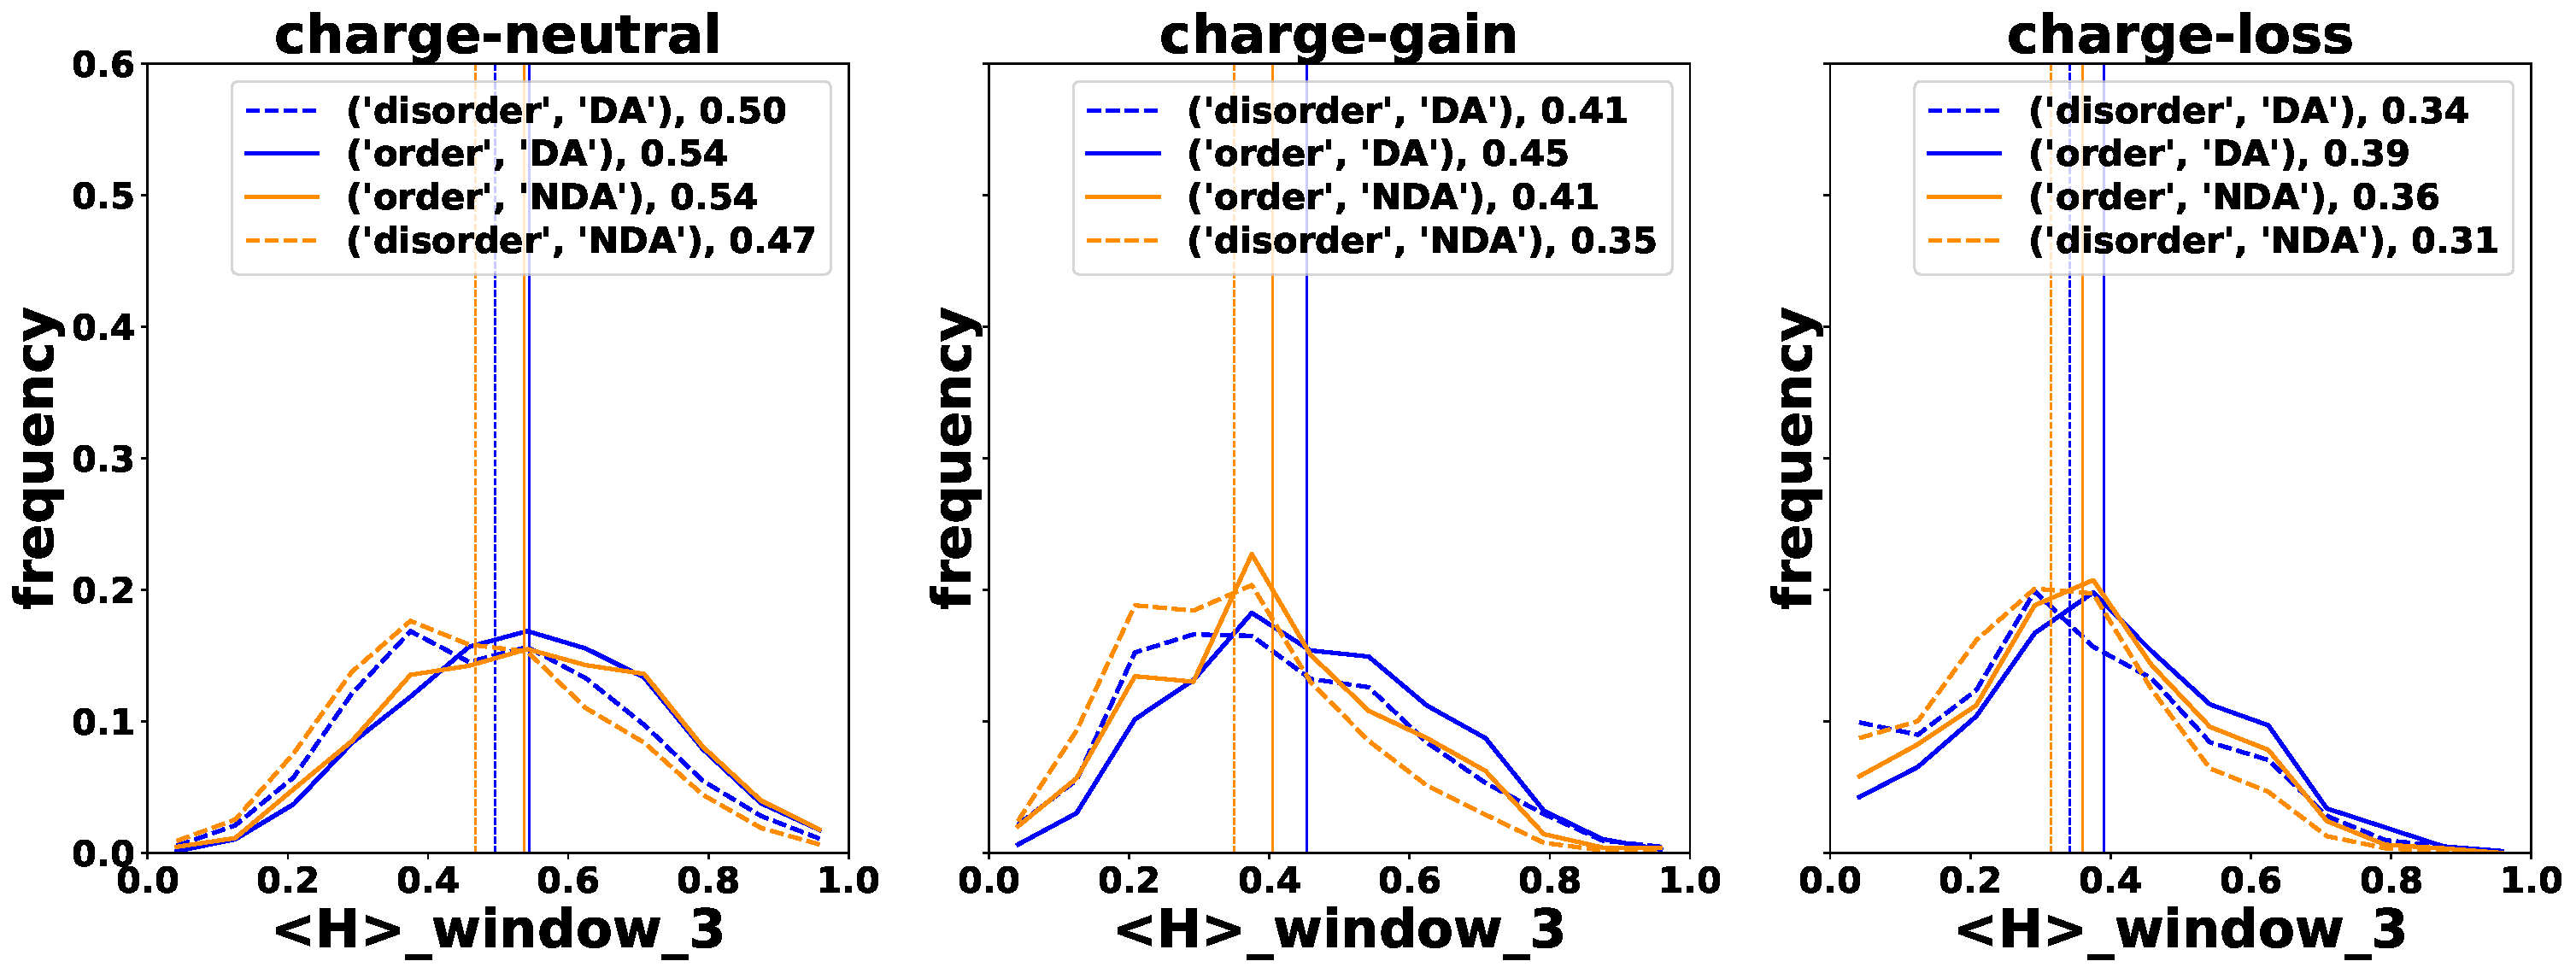
\includegraphics[scale=0.1,width=\textwidth,trim={0 0cm 0 0cm},clip]{./figures/snp_hydropathy_distribution_3.pdf}
\caption{{\bf DA SNPs are more enriched in hydrophobic regions.} We looked at the hydrophobicity distribution of SNP residue and it's neighboring residue. The mean of each histogram distribution is also reported in caption. We find that DA SNPs are found in hydrophobic regions when compared with NDA SNPs in both ordered and disordered proteins.}
\label{fig2} 
\end{figure}

\begin{figure}[!ht]
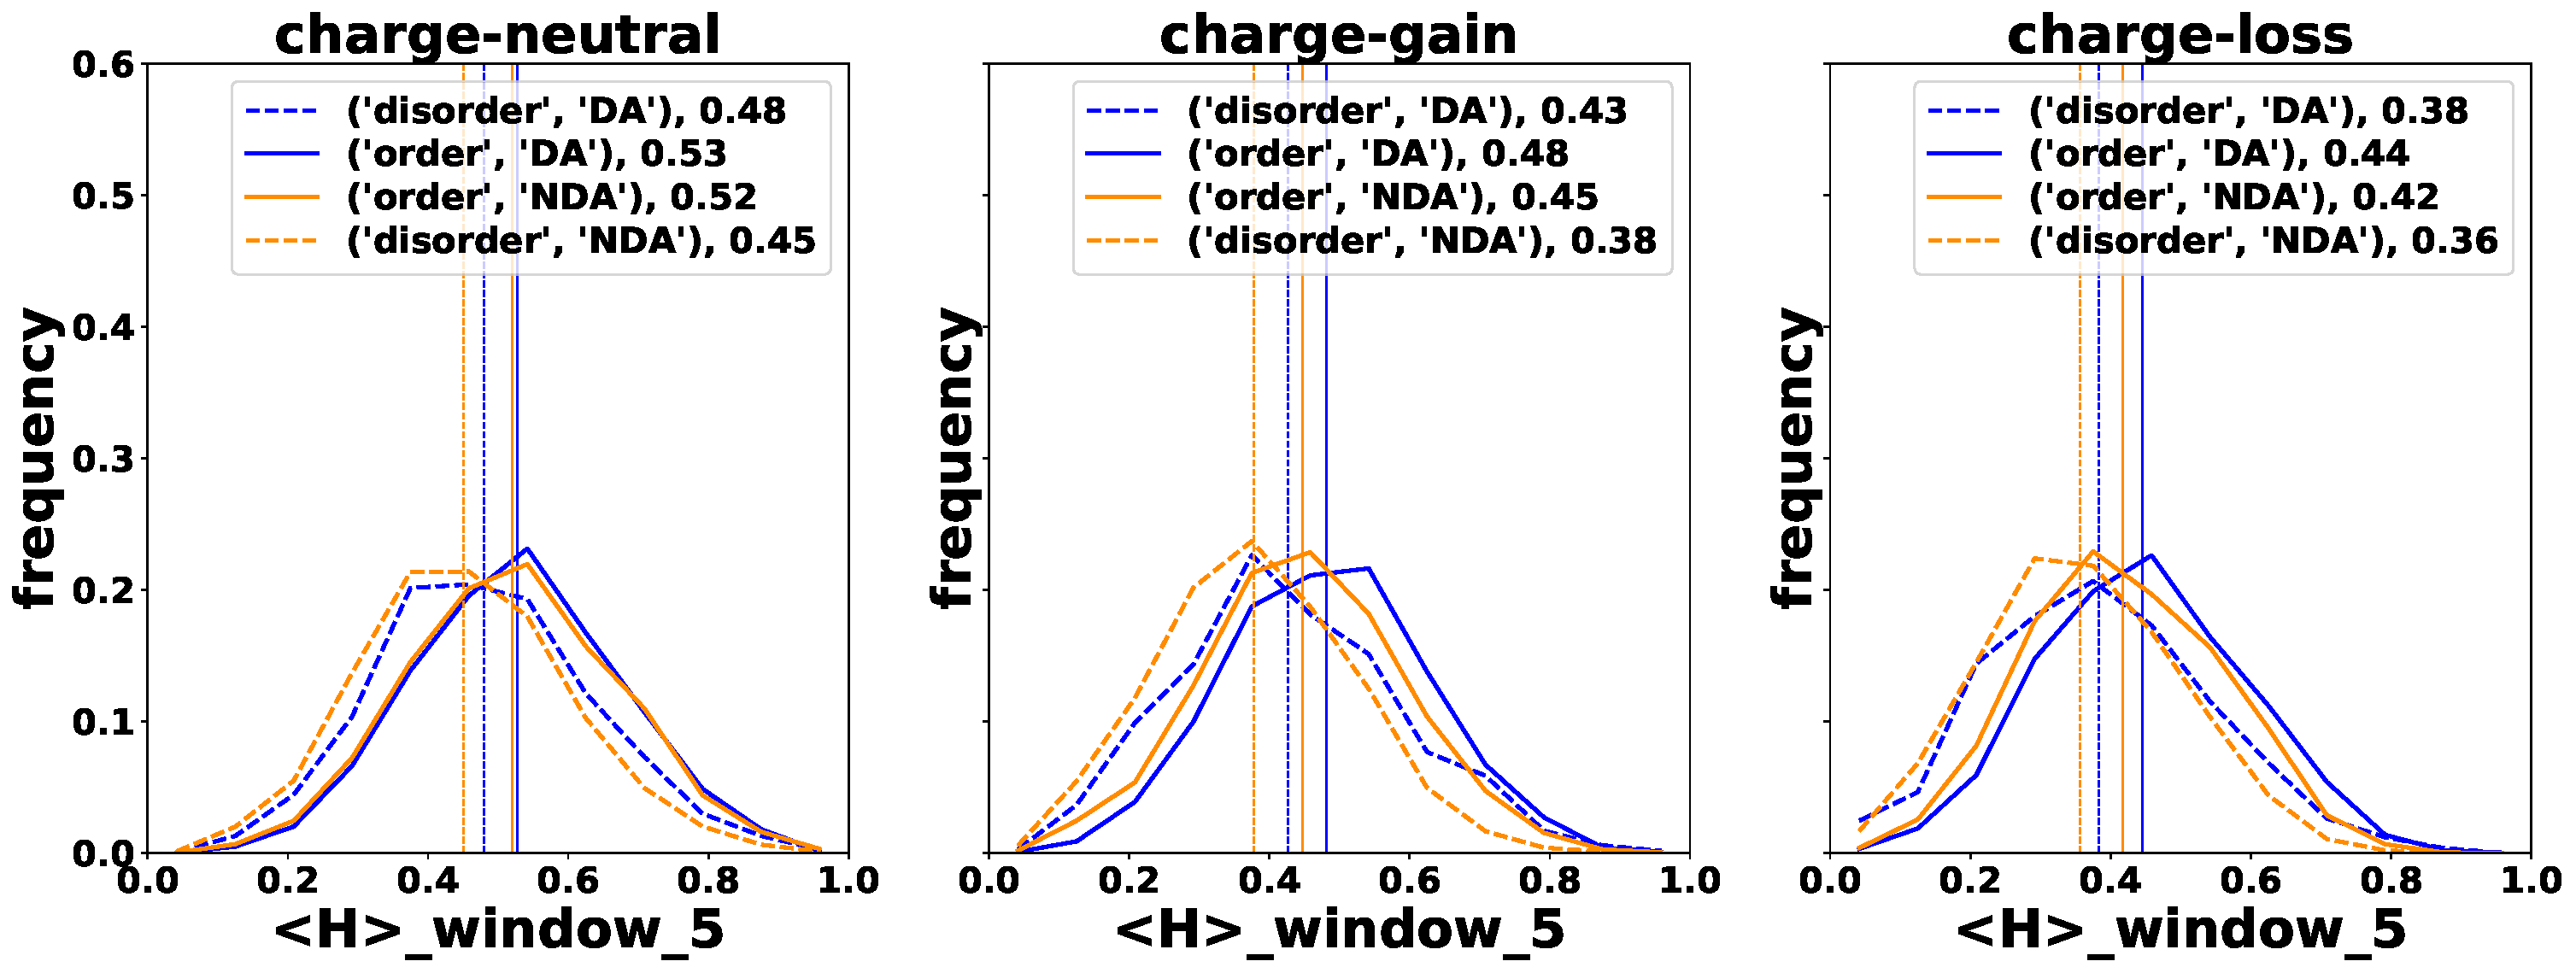
\includegraphics[scale=0.1,width=1\textwidth,trim={0 0cm 0 0cm},clip]{./figures/snp_hydropathy_distribution_5.pdf}
\caption{{\bf DA SNPs are more enriched in hydrophobic regions.} Same as Fig 3 but with window size 5 instead of 3. }
\label{fig3} 
\end{figure}

\begin{figure}[!ht]
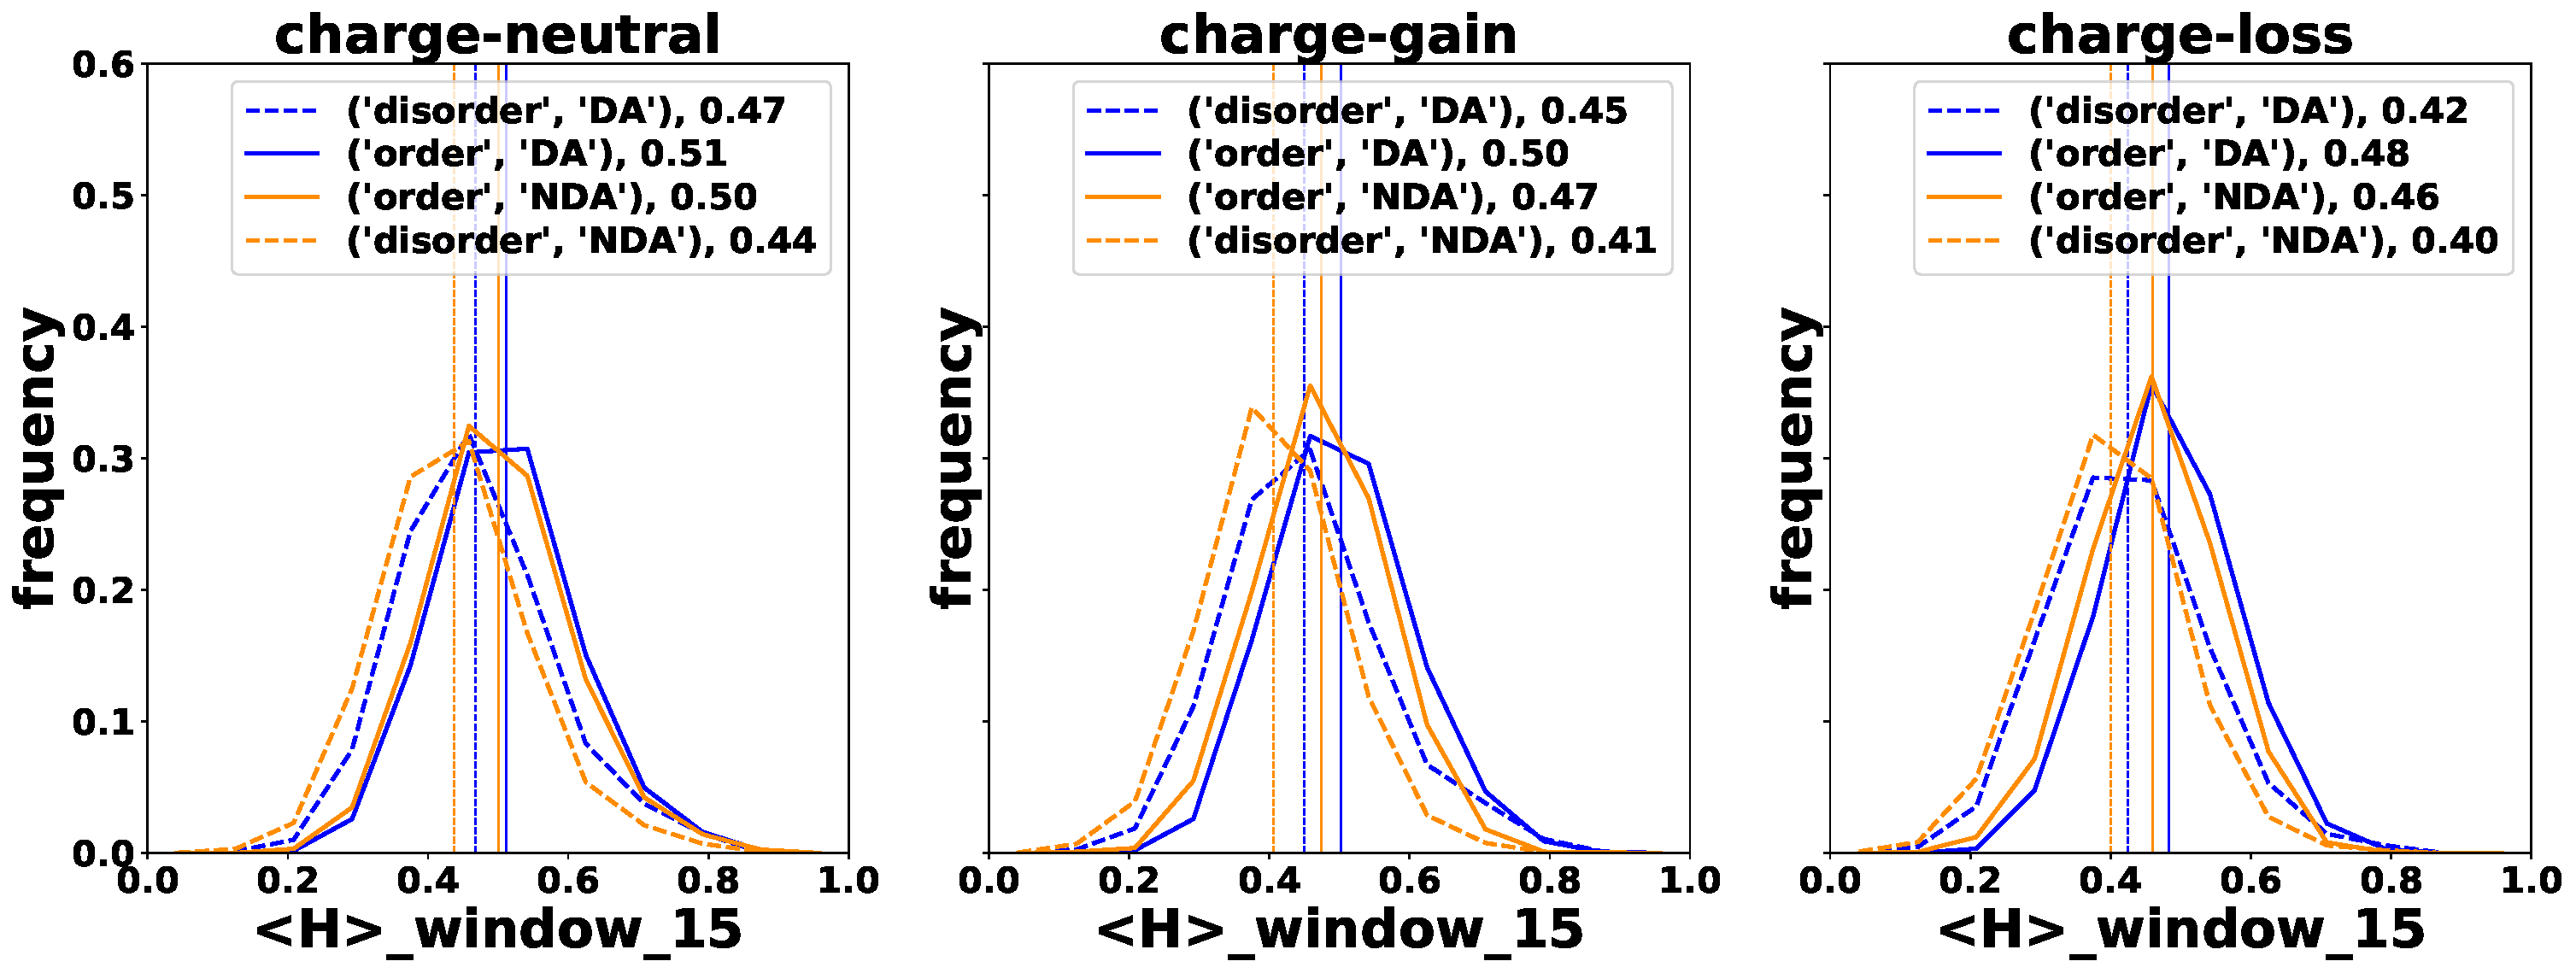
\includegraphics[scale=0.1,width=\textwidth,trim={0 0cm 0 0cm},clip]{./figures/snp_hydropathy_distribution_15.pdf}
\caption{{\bf DA SNPs are more enriched in hydrophobic regions.} Same as Fig 3 but with window size 15 instead of 3. }
\label{fig4} 
\end{figure}

\clearpage
\subsection*{DA SNPs are enriched in hydrophobic domains}
\bigbreak
The sequence was divided into hydrophobic domains as described in Methods. We find that DA SNPs are enriched in h domains in both ordered and disordered proteins.  
\begin{figure}[!ht]
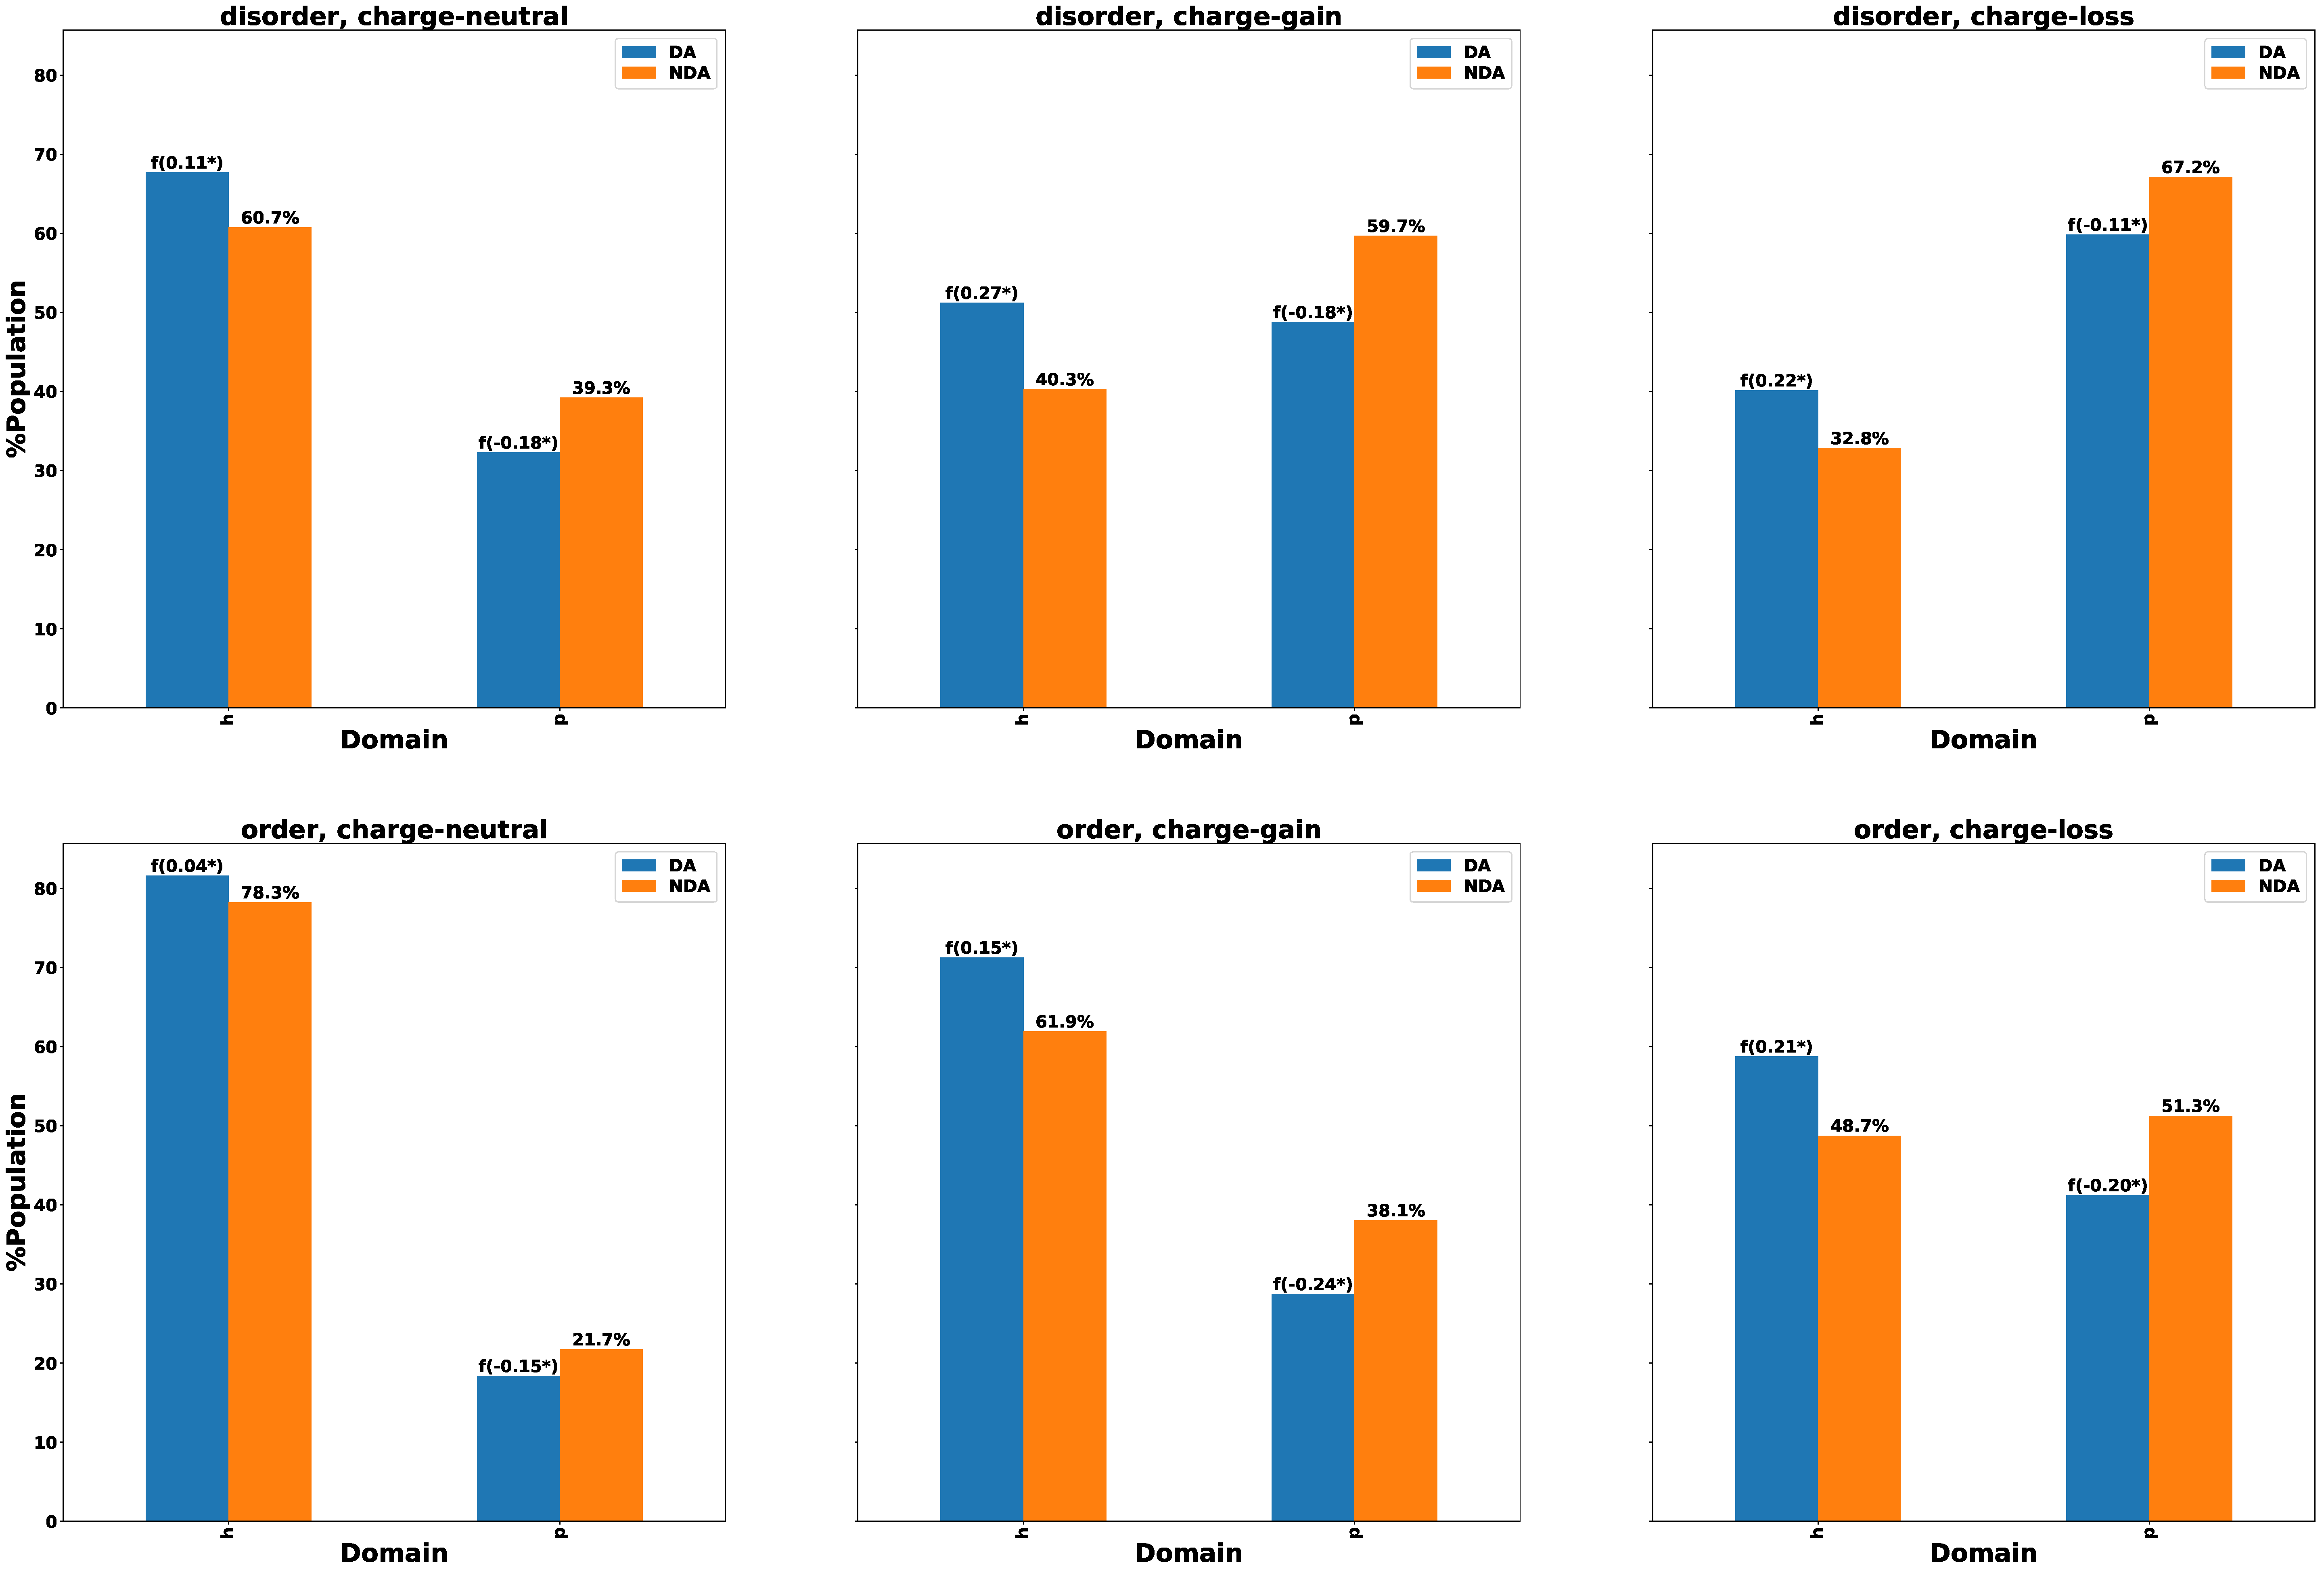
\includegraphics[scale=0.1,width=\textwidth,trim={0 0cm 0 0cm},clip]{./figures/charge_vs_no_charge_order_vs_disorder_SNP_Domain.pdf}
\caption{{\bf DA SNPs are enriched in hydrophobic domains. Cutoff-0.37} We looked at the population of SNPs in hydrophobic domains (h) and linker regions (p). The top and bottom panel is for disordered and ordered regions respectively. The sequence was divided into hydrophobic domains as described in Methods. We find that DA SNPs are enriched in h domains in both ordered and disordered proteins.Fold enrichment in DA SNPs when compared with not-disease-associated SNPs is annotated in the plot as well with f. If p-value from the binomial test is $<$ .005, the enrichment is marked with star.}
\label{fig5} 
\end{figure}


\begin{figure}[!ht]
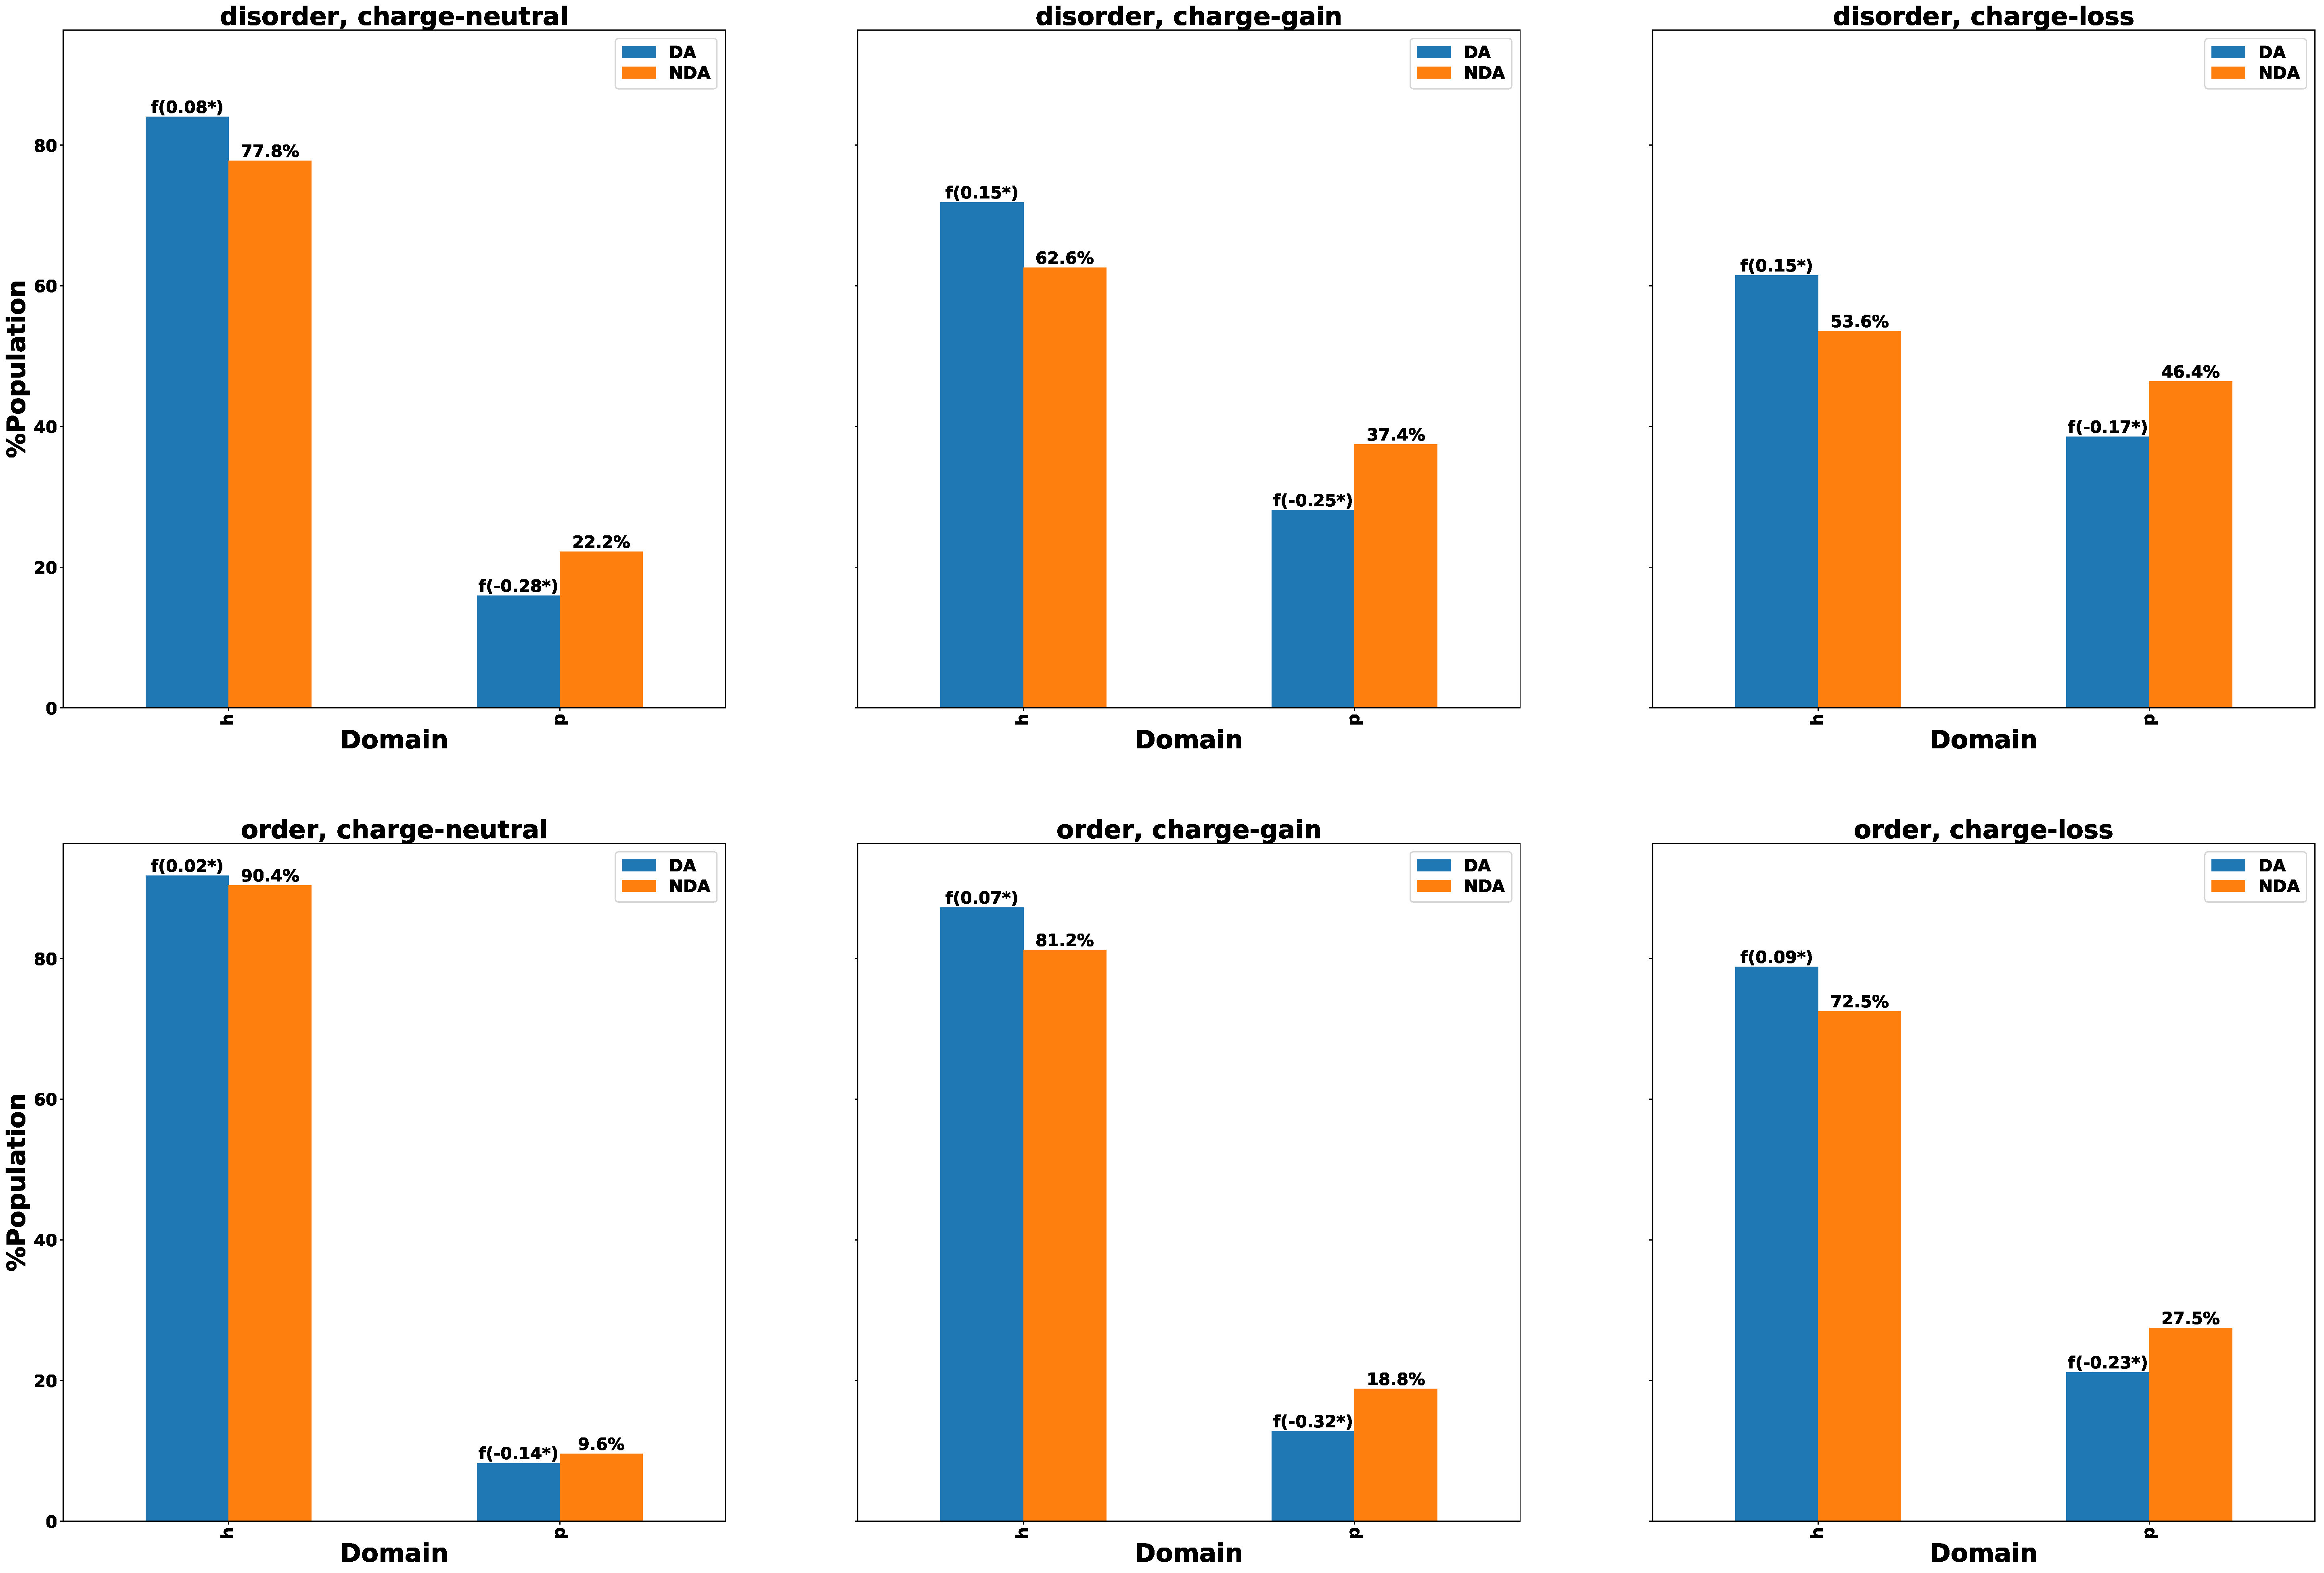
\includegraphics[scale=0.1,width=\textwidth,trim={0 0cm 0 0cm},clip]{./figures/charge_vs_no_charge_order_vs_disorder_SNP_Domain_three.pdf}
\caption{{\bf DA SNPs are enriched in hydrophobic domains. Cutoff-0.3} . Same as Fig 5 but with cutoff 0.3.}
\label{fig5} 
\end{figure}

\begin{figure}[!ht]
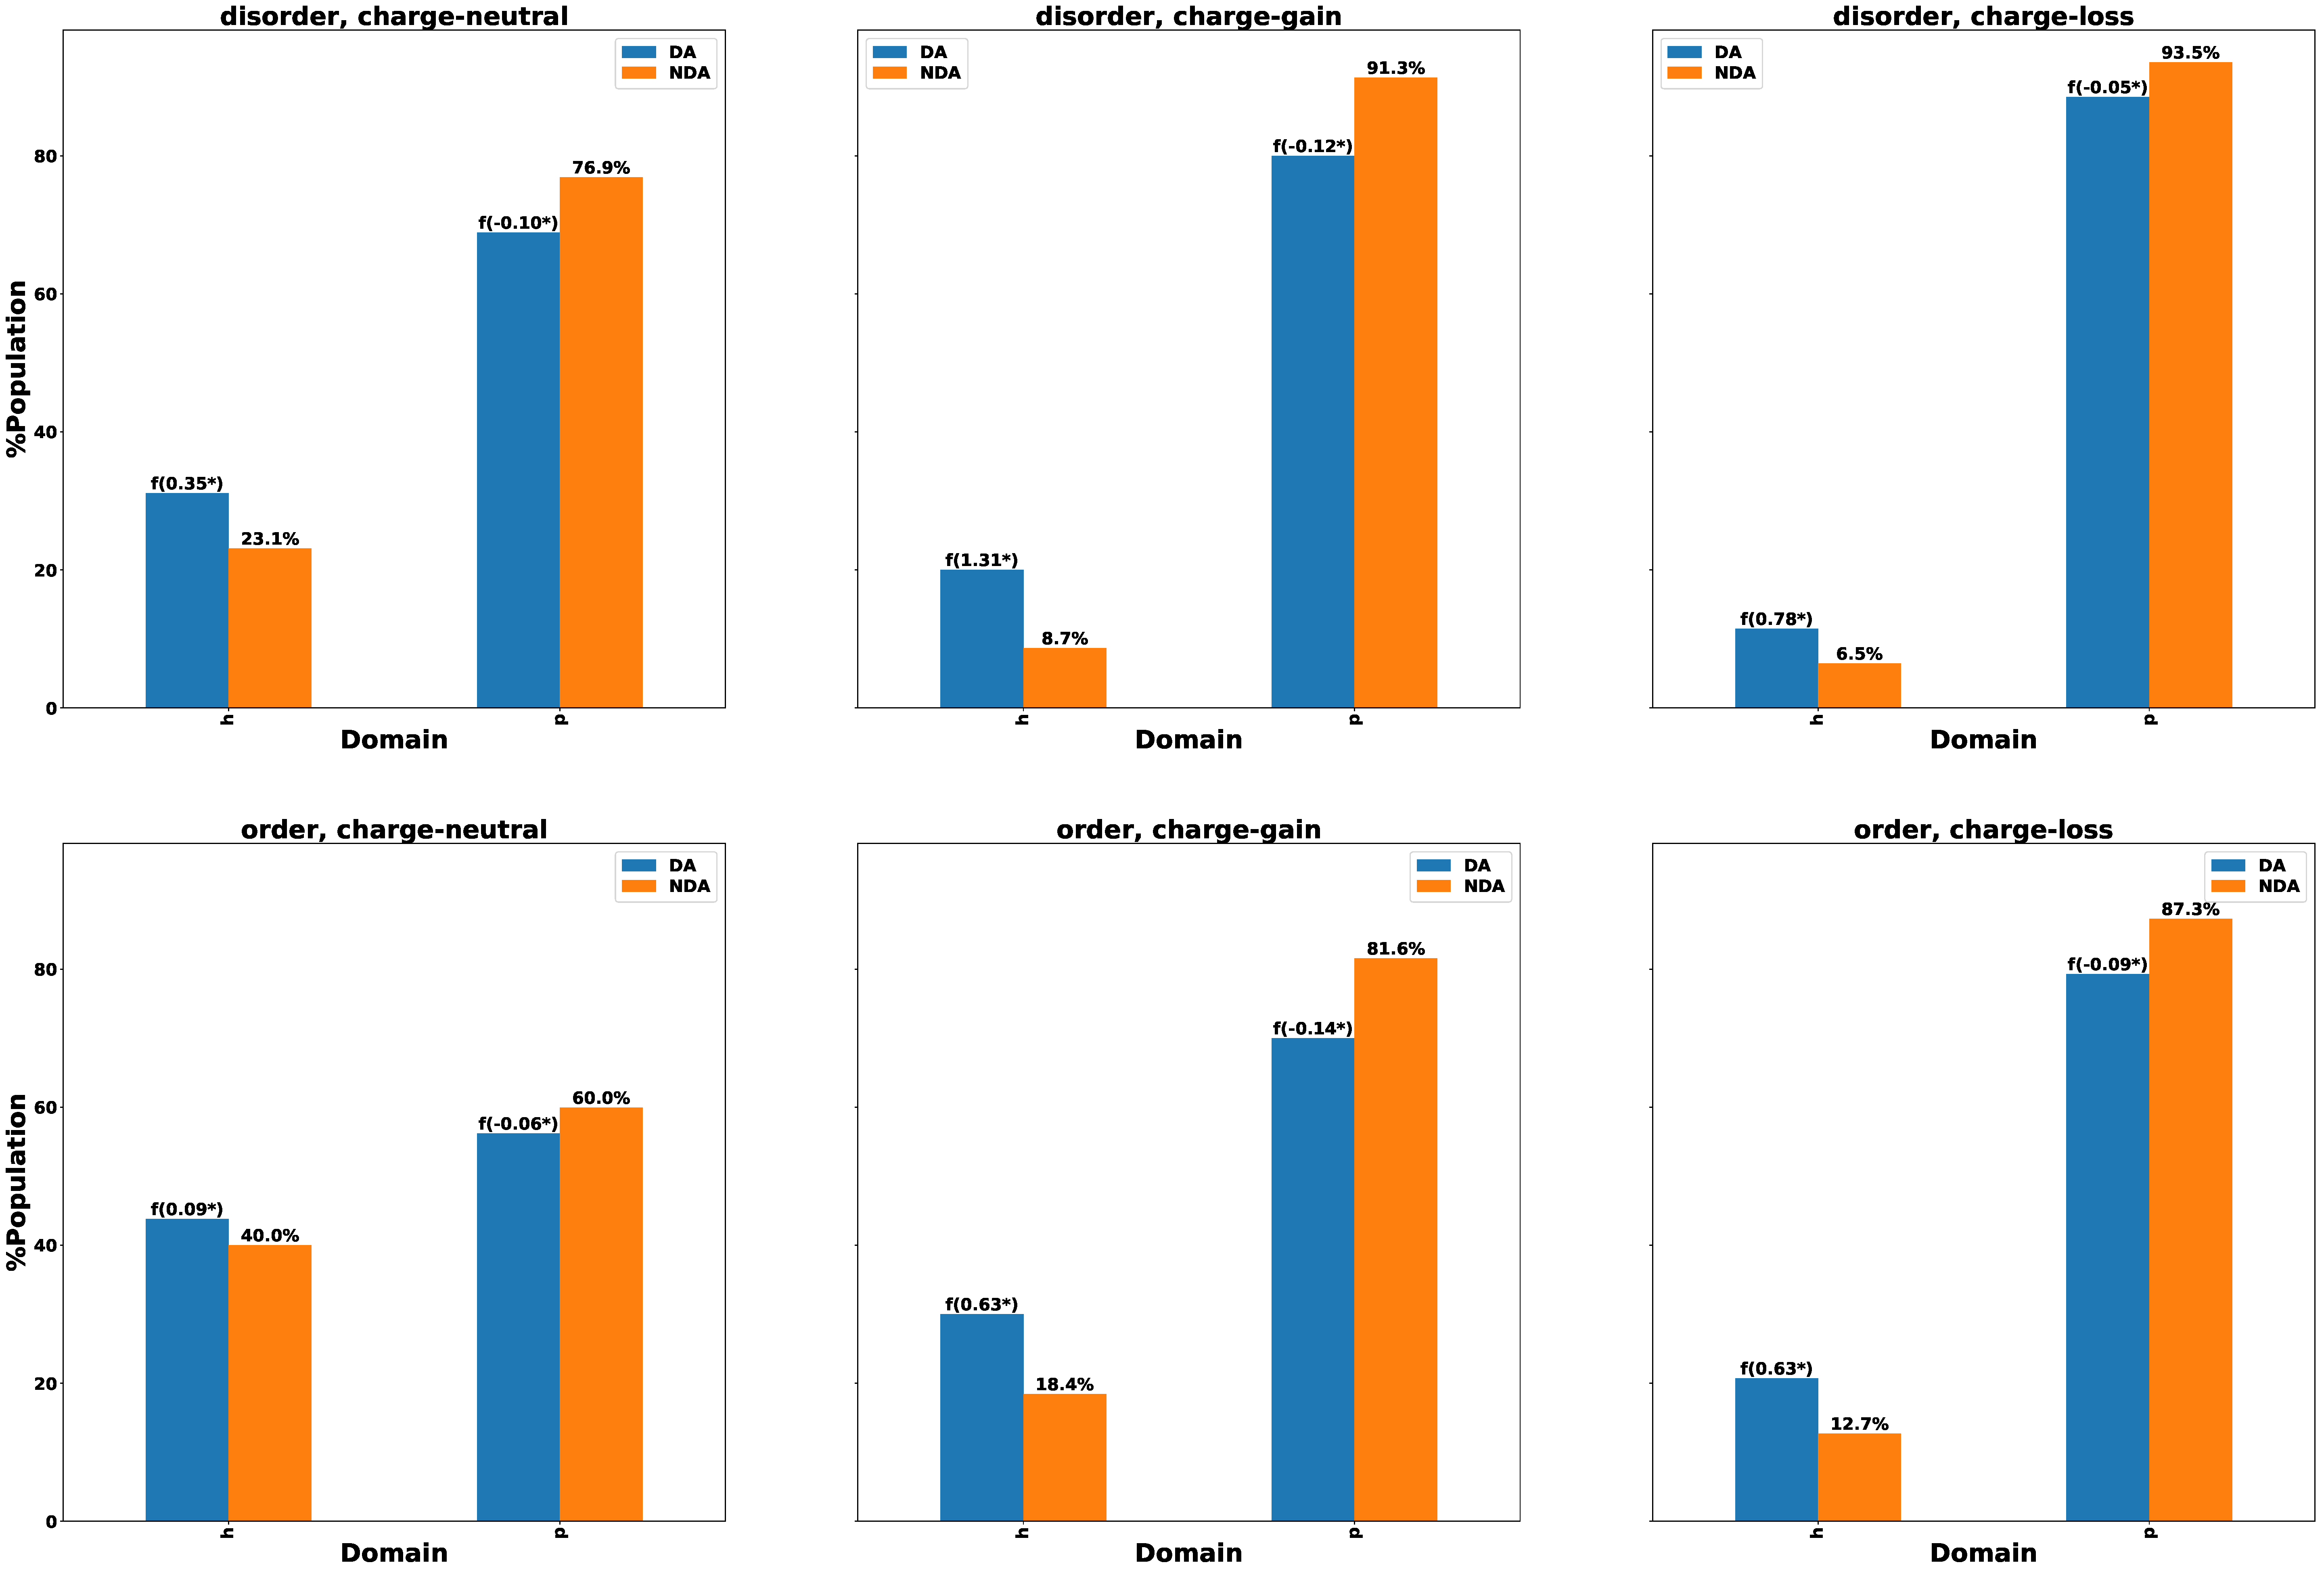
\includegraphics[scale=0.1,width=\textwidth,trim={0 0cm 0 0cm},clip]{./figures/charge_vs_no_charge_order_vs_disorder_SNP_Domain_five.pdf}
\caption{{\bf DA SNPs are enriched in hydrophobic domains. Cutoff-0.5}. Same as Fig 5 but with cutoff 0.5.}
\label{fig5} 
\end{figure}

\clearpage
\subsection*{Mutations change hydrophobic regions to less hydrophobic regions/ domain transformation}

We find that SNPs are enriched in conversion of a hydrophobic domain to a linker region in both ordered and disordered proteins. 
\begin{figure}[!ht]
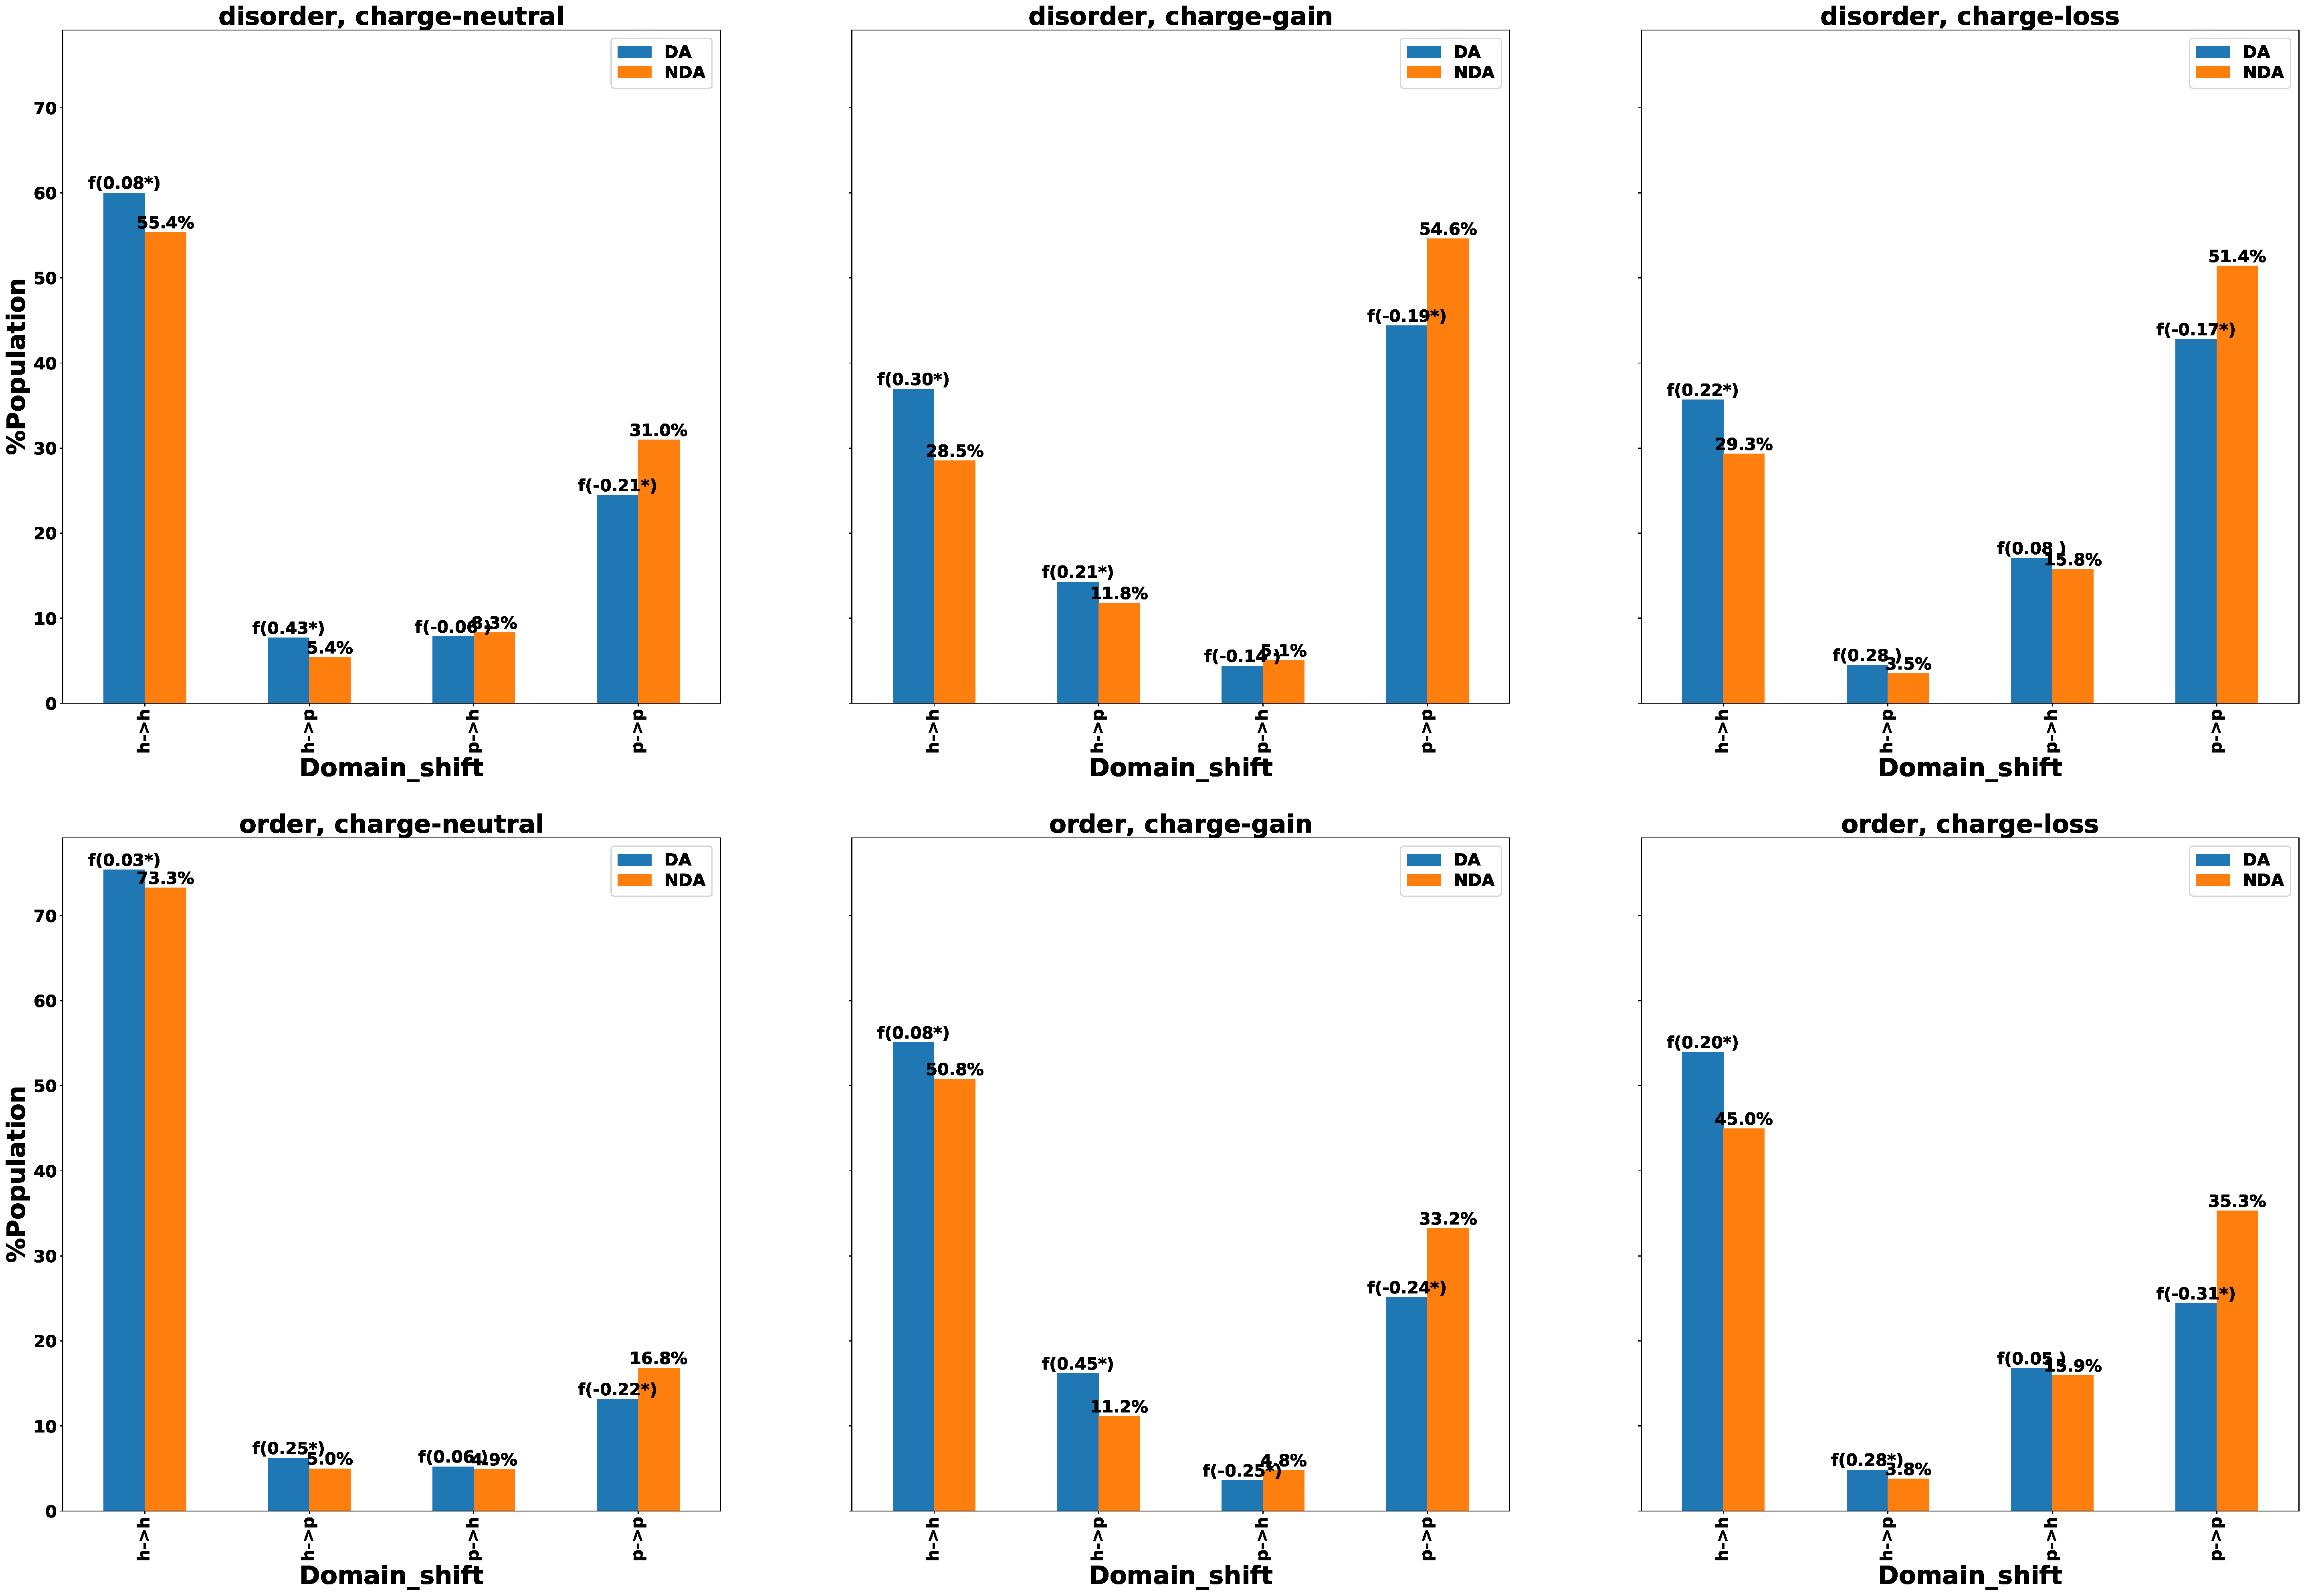
\includegraphics[scale=0.1,width=\textwidth,trim={0 0cm 0 0cm},clip]{./figures/charge_vs_no_charge_order_vs_disorder_SNP_Domain_shift.pdf}
\caption{{\bf DA SNPs change hydrophobic regions to less hydrophobic regions.} We looked at the populations of domain change associated with each SNPs in each category. DA SNPs in hydrophobic domains are enriched in changing these hydrophobic domains (h) to linker regions (p) relative to NDA SNPs in both disordered and ordered proteins. The top and bottom panel is for disordered and ordered regions respectively. Fold enrichment in DA SNPs when compared with not-disease-associated SNPs is annotated in the plot as well with f. If p-value from the binomial test is $<$ .005, the enrichment is marked with star.}
\label{fig6} 
\end{figure}


\clearpage
\subsection*{The addition of Methionine}
We find that the addition of methionine is highly enriched with DA SNPs. 
\begin{figure}[!ht]
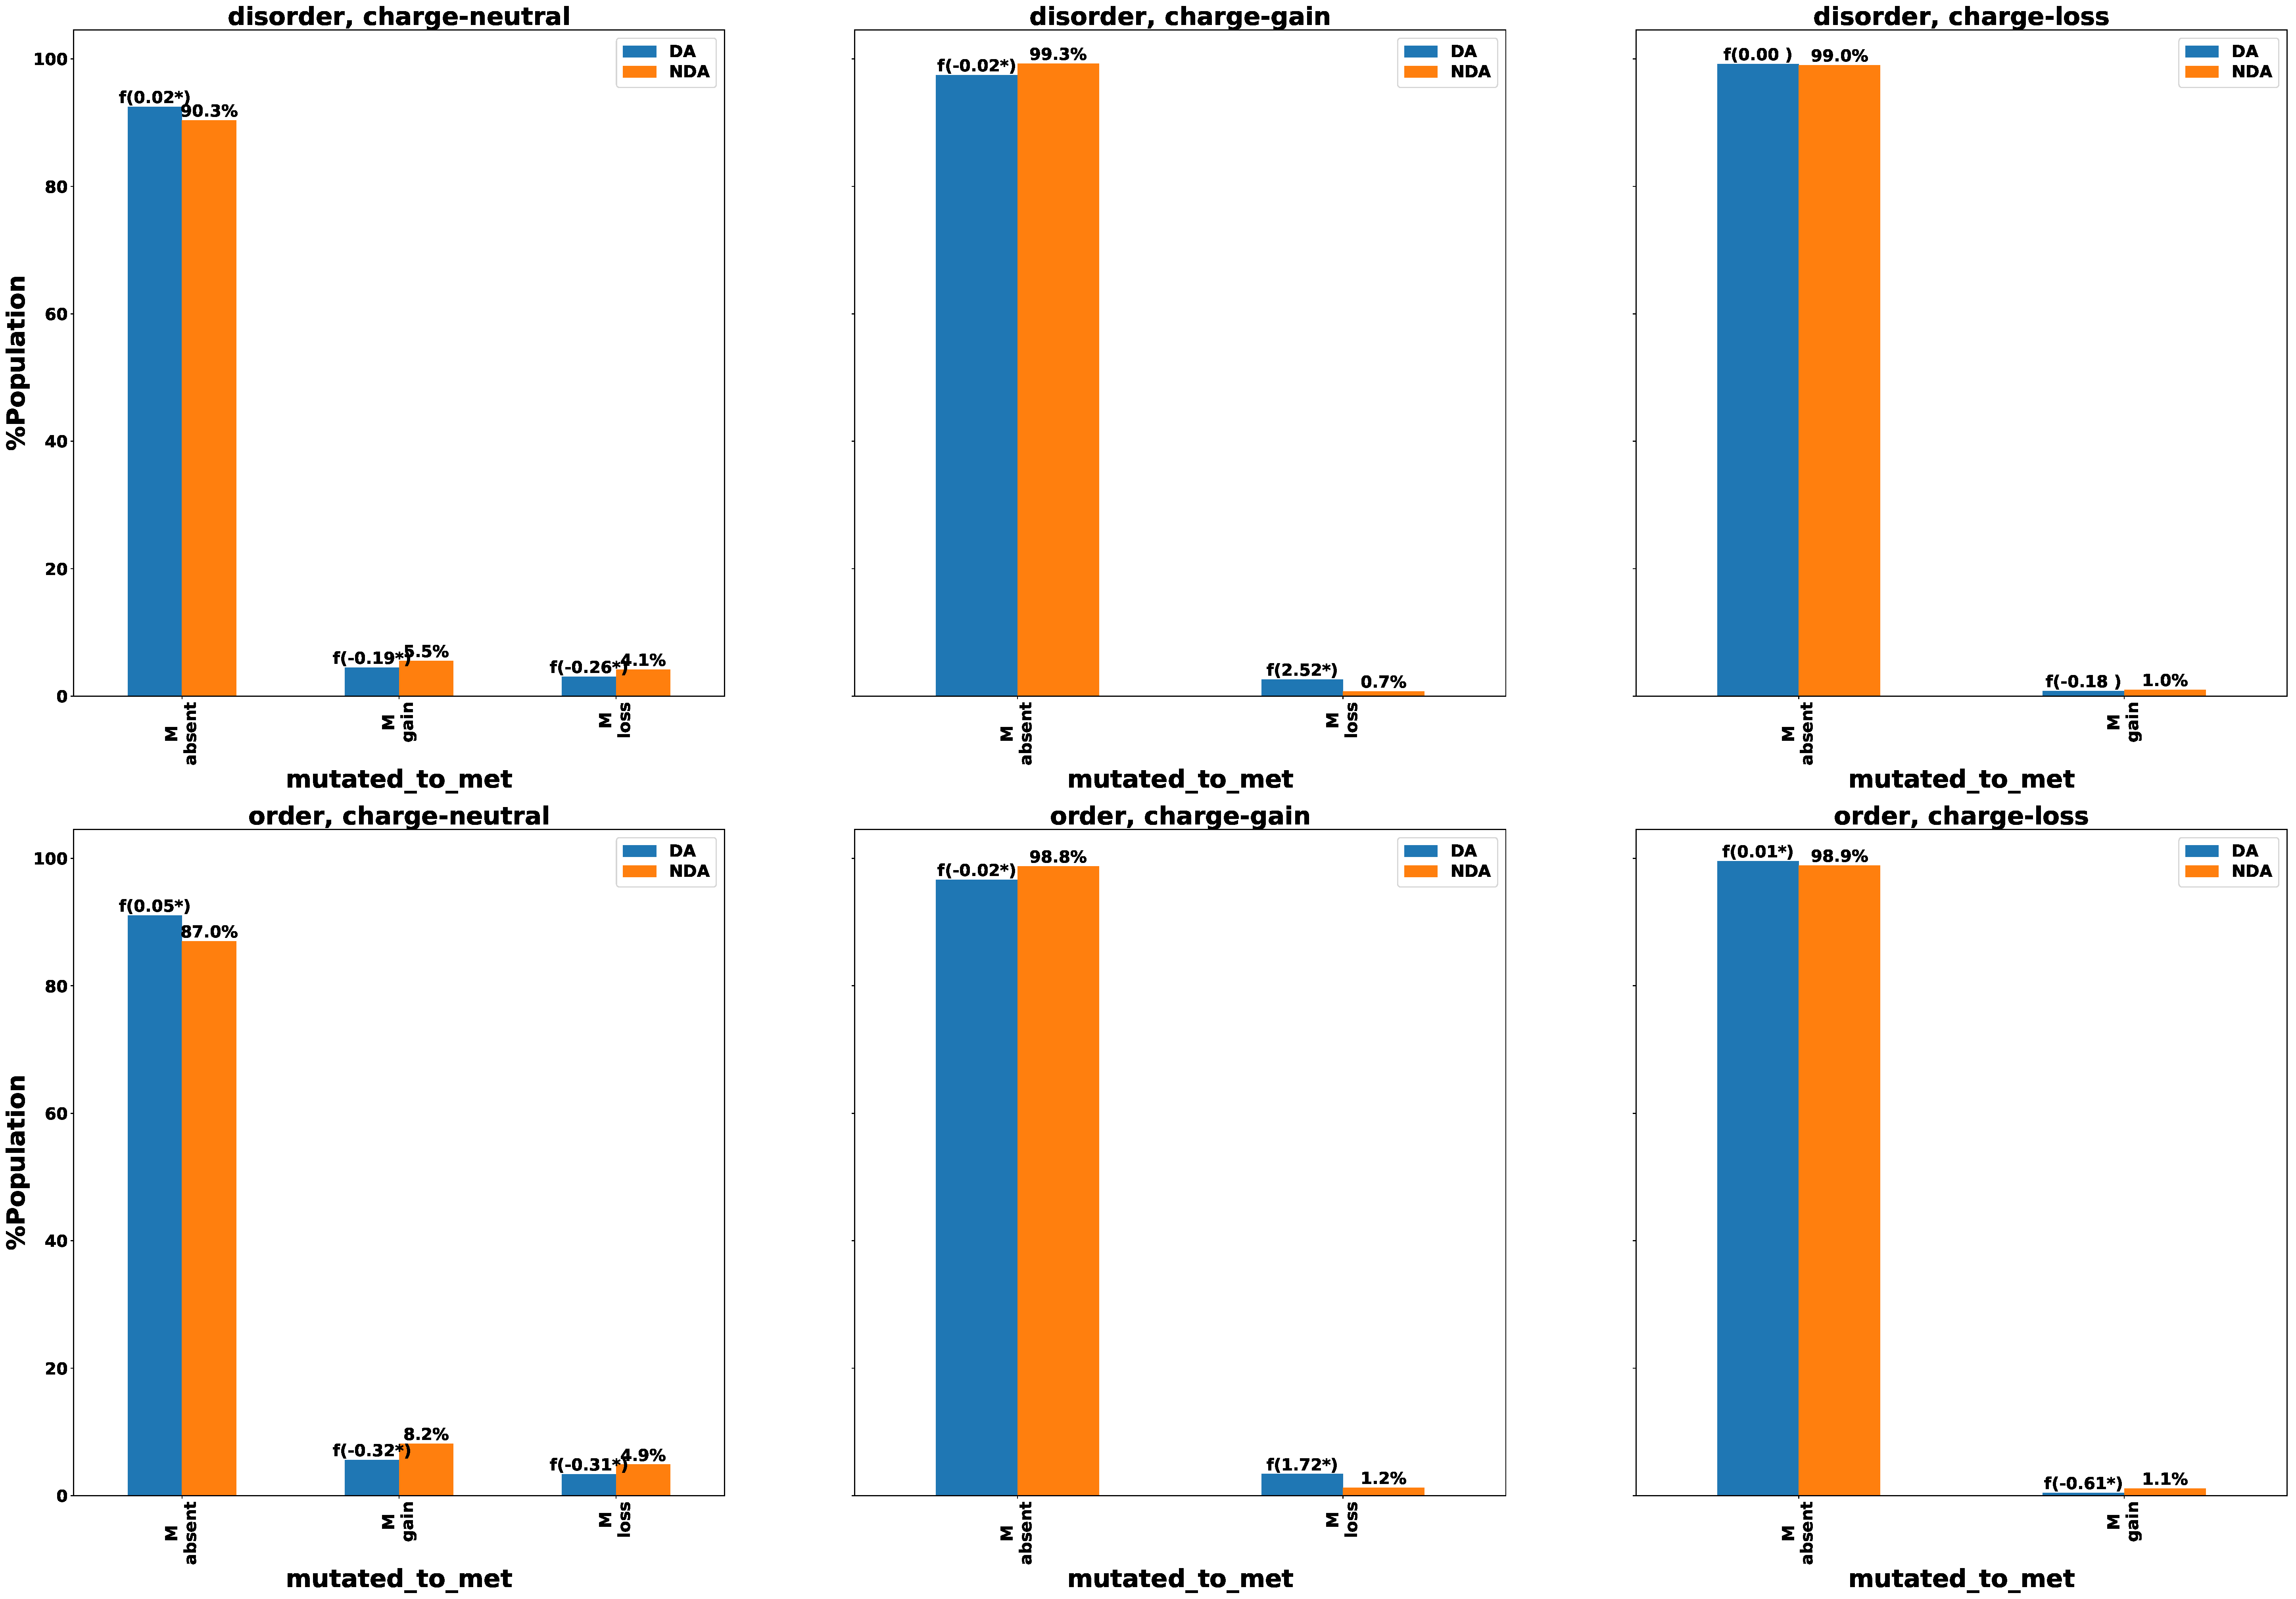
\includegraphics[scale=0.1,width=\textwidth,trim={0 0cm 0 0cm},clip]{./figures/charge_vs_no_charge_order_vs_disorder_SNP_mutated_to_met.pdf}
\caption{{\bf DA SNPs are enriched in hydrophobic domains.} We looked at whether at whether Met gain or loss is associated with diseases. We find that loss of Met and gain of charge is enriched in DA when compared with NDA SNPs}
\label{fig5} 
\end{figure}
\bigbreak
\subsection*{Few example of domain and SNP identification in proteins.}
\bigbreak
\subsection*{The online tool for analyzing your own protein sequence :)}
\bigbreak
\section*{Materials and Methods}

\subsection*{Datasets}
The list of all missense variants annotated in human UniProtKB/Swiss-Prot entries was obtained from http://beta.uniprot.org/docs/humsavar (last Release: 8th May 2019)~\cite{Yip2008a}. This manually curated catalog contains missense mutations on the most common isoform of the given protein and does not contain frameshift and nonsense mutation. A variant is annotated as `Disease' or `Polymorphisms' depending on if it is implicated in disease or not according to literature reports. `Polymorphisms' is also used to describe rare variants as well as polymorphisms that have an effect on protein function, but with no resulting clinical phenotype (functional polymorphisms)~\cite{Yip2008a}. A total number of 78,678 missense mutations were found in the database, among which 30,597 (38.9\%) are associated to diseases, 40,032 (50.1\%) are polymorphisms, and 1,973 (10.2\%) are still unclassified. 

The initial set of mutations was filtered as follows: The proteins associated with disease mutations were clustered using UniRef50~\cite{Suzek2015}. Only one protein from each cluster was selected. `Polymorphisms' dataset was analogously filtered as well. We further removed three proteins with an unusually high number of annotated disease mutations (UniProtKB: P35555, P35498, P00451).

Protein disorder for wild type sequences was obtained from Database of Disordered Protein Prediction (D2P2) (http://d2p2.pro). D2P2 has disorder predicted from nine disorder predictor including PONDR VL-XT, PONDR VSL2b, PrDOS, PV2, Espritz (all variants) and IUPred (all variants)~\cite{Oates2012}. We annotated any residue as disordered if at-least two disorder predictor predicts it be disordered. 

\subsection*{Domain identification} Mean hydrophobicity ($\langle H\rangle$) at each residue is defined as the average Kyte-Dolittle\cite{Kyte1982a} score with a window size of 3 residues, scaled to fit between 0 and 1. Any stretch of four or more residues with $\langle H \rangle$ $>$ 0.37 is classified as hydrophobic domain and from the remaining residues, stretch of four or more residues is classified as linker region.


\section*{Acknowledgments}


\section*{Supporting Information}



% Either type in your references using
% Either type in your references using
% \begin{thebibliography}{}
% \bibitem{}
% Text
% \end{thebibliography}
%
% or
%
% Compile your BiBTeX database using our plos2015.bst
% style file and paste the contents of your .bbl file
% here.

\bibliography{bioinfo-scan}
\end{document}
